% A LaTeX template for MSc Thesis submissions to 
% Politecnico di Milano (PoliMi) - School of Industrial and Information Engineering
%
% S. Bonetti, A. Gruttadauria, G. Mescolini, A. Zingaro
% e-mail: template-tesi-ingind@polimi.it
%
% Last Revision: October 2021
%
% Copyright 2021 Politecnico di Milano, Italy. NC-BY

\documentclass{Configuration_Files/PoliMi3i_thesis}

%------------------------------------------------------------------------------
%	REQUIRED PACKAGES AND  CONFIGURATIONS
%------------------------------------------------------------------------------

% CONFIGURATIONS
\usepackage{parskip} % For paragraph layout
\usepackage{setspace} % For using single or double spacing
\usepackage{emptypage} % To insert empty pages
\usepackage{multicol} % To write in multiple columns (executive summary)
\setlength\columnsep{15pt} % Column separation in executive summary
\setlength\parindent{0pt} % Indentation
\raggedbottom

% PACKAGES FOR TITLES
\usepackage{titlesec}
% \titlespacing{\section}{left spacing}{before spacing}{after spacing}
\titlespacing{\section}{0pt}{3.3ex}{2ex}
\titlespacing{\subsection}{0pt}{3.3ex}{1.65ex}
\titlespacing{\subsubsection}{0pt}{3.3ex}{1ex}
\usepackage{color}

% PACKAGES FOR LANGUAGE AND FONT
\usepackage[english]{babel} % The document is in English  
\usepackage[utf8]{inputenc} % UTF8 encoding
\usepackage[T1]{fontenc} % Font encoding
\usepackage[11pt]{moresize} % Big fonts

% PACKAGES FOR IMAGES
\usepackage{graphicx}
\usepackage{transparent} % Enables transparent images
\usepackage{eso-pic} % For the background picture on the title page
\usepackage{subfig} % Numbered and caption subfigures using \subfloat.
\usepackage{tikz} % A package for high-quality hand-made figures.
\usetikzlibrary{}
\graphicspath{{./Images/}} % Directory of the images
\usepackage{amsthm} % Coloured "Theorem"
\usepackage{thmtools}
\usepackage{xcolor}
\usepackage{float}

% STANDARD MATH PACKAGES
\usepackage{amsmath}
\usepackage{amssymb}
\usepackage{amsfonts}
\usepackage{bm}
\usepackage[overload]{empheq} % For braced-style systems of equations.
\usepackage{fix-cm} % To override original LaTeX restrictions on sizes

% PACKAGES FOR TABLES
\usepackage{tabularx}
\usepackage{longtable} % Tables that can span several pages
\usepackage{colortbl}

% PACKAGES FOR ALGORITHMS (PSEUDO-CODE)
\usepackage{algorithm}
\usepackage{algorithmic}

% PACKAGES FOR REFERENCES & BIBLIOGRAPHY
\usepackage[
    colorlinks=true,
    linkcolor=black,
    anchorcolor=black,
    citecolor=black,
    filecolor=black,
    menucolor=black,
    runcolor=black,
    urlcolor=black
]{hyperref} % Adds clickable links at references
\usepackage{cleveref}
\usepackage[square, numbers, sort&compress]{natbib} % Square brackets, citing references with numbers, citations sorted by appearance in the text and compressed
\bibliographystyle{abbrvnat} % You may use a different style adapted to your field

% OTHER PACKAGES
\usepackage{pdfpages} % To include a pdf file
\usepackage{afterpage}
\usepackage{lipsum} % DUMMY PACKAGE
\usepackage{fancyhdr}
\usepackage{wasysym} % For the headers

\usepackage{listings}
%%
% Alloy language definition for using with the listings package.
%
% 2017, Daniel Andrade
% BSD 3-Clause License
%%
\lstdefinelanguage{alloy}{
    morekeywords={
        module, open, as,
        private, abstract, sig, extends, in,
        lone, some, one, disj,
        fact, pred, fun, assert,
        run, check,
        for, but, exactly,
        this, not, implies, else, let,
        not, no, set, all, sum,
        iff, or, Int, and,
        none, univ, iden
    },
    sensitive=true,
    morecomment=[l]{//},
    morecomment=[l]{--},
    morecomment=[s]{/*}{*/},
    morestring=[b]{"},
%literate={->}{$\rightarrow$}1
% replacing characters can cause problems when copying from PDF to editor
}[keywords,comments,strings]

\lstdefinestyle{alloy}{
    commentstyle=\itshape,
    keywordstyle=\bfseries,
    stringstyle=\itshape,
}

%\definecolor{dkgreen}{rgb}{0,0.6,0}
%\definecolor{gray}{rgb}{0.5,0.5,0.5}
%\definecolor{mauve}{rgb}{0.58,0,0.82}

%\lstset{frame=tb,
%    language=Alloy,
%    aboveskip=3mm,
%    belowskip=3mm,
%    showstringspaces=false,
%    columns=flexible,
%    basicstyle={\small\ttfamily},
%    numbers=none,
%    numberstyle=\tiny\color{gray},
%    keywordstyle=\color{blue},
%    commentstyle=\color{dkgreen},
%    stringstyle=\color{mauve},
%    breaklines=true,
%    breakatwhitespace=true,
%    tabsize=3
%}



\fancyhf{}

% Input of configuration file. Do not change config.tex file unless you really know what you are doing. 
% Define blue color typical of polimi
\definecolor{bluepoli}{cmyk}{0.4,0.1,0,0.4}

% Custom theorem environments
\declaretheoremstyle[
    headfont=\color{bluepoli}\normalfont\bfseries,
    bodyfont=\color{black}\normalfont\itshape,
]{colored}

% Set-up caption colors
\captionsetup[figure]{labelfont={color=bluepoli}} % Set colour of the captions
\captionsetup[table]{labelfont={color=bluepoli}} % Set colour of the captions
\captionsetup[algorithm]{labelfont={color=bluepoli}} % Set colour of the captions

\theoremstyle{colored}
\newtheorem{theorem}{Theorem}[chapter]
\newtheorem{proposition}{Proposition}[chapter]

% Enhances the features of the standard "table" and "tabular" environments.
\newcommand\T{\rule{0pt}{2.6ex}}
\newcommand\B{\rule[-1.2ex]{0pt}{0pt}}

% Pseudo-code algorithm descriptions.
\newcounter{algsubstate}
\renewcommand{\thealgsubstate}{\alph{algsubstate}}
\newenvironment{algsubstates}
{\setcounter{algsubstate}{0}%
\renewcommand{\STATE}{%
    \stepcounter{algsubstate}%
    \Statex {\small\thealgsubstate:}\space}}
{}

% New font size
\newcommand\numfontsize{\@setfontsize\Huge{200}{60}}

% Title format: chapter
\titleformat{\chapter}[hang]{
    \fontsize{50}{20}\selectfont\bfseries\filright}{\textcolor{bluepoli} \thechapter\hsp\hspace{2mm}\textcolor{bluepoli}{|   }\hsp}{0pt}{\huge\bfseries \textcolor{bluepoli}
}

% Title format: section
\titleformat{\section}
{\color{bluepoli}\normalfont\Large\bfseries}
{\color{bluepoli}\thesection.}{1em}{}

% Title format: subsection
\titleformat{\subsection}
{\color{bluepoli}\normalfont\large\bfseries}
{\color{bluepoli}\thesubsection.}{1em}{}

% Title format: subsubsection
\titleformat{\subsubsection}
{\color{bluepoli}\normalfont\large\bfseries}
{\color{bluepoli}\thesubsubsection.}{1em}{}

% Shortening for setting no horizontal-spacing
\newcommand{\hsp}{\hspace{0pt}}

\makeatletter
% Renewcommand: cleardoublepage including the background pic
\renewcommand*\cleardoublepage{%
    \clearpage\if@twoside\ifodd\c@page\else
    \null
    \AddToShipoutPicture*{\BackgroundPic}
    \thispagestyle{empty}%
    \newpage
    \if@twocolumn\hbox{}\newpage\fi\fi\fi}
\makeatother

%For correctly numbering algorithms
\numberwithin{algorithm}{chapter}

%----------------------------------------------------------------------------
%	NEW COMMANDS DEFINED
%----------------------------------------------------------------------------

%----------------------------------------------------------------------------
%	ADD YOUR PACKAGES (be careful of package interaction)
%----------------------------------------------------------------------------

%----------------------------------------------------------------------------
%	ADD YOUR DEFINITIONS AND COMMANDS (be careful of existing commands)
%----------------------------------------------------------------------------

%----------------------------------------------------------------------------
%	BEGIN OF YOUR DOCUMENT
%----------------------------------------------------------------------------

\begin{document}
    \fancypagestyle{plain}{%
        \fancyhf{} % Clear all header and footer fields
        \fancyhead[RO,RE]{\thepage} %RO=right odd, RE=right even
        \renewcommand{\headrulewidth}{0pt}
        \renewcommand{\footrulewidth}{0pt}}

%----------------------------------------------------------------------------
%	TITLE PAGE
%----------------------------------------------------------------------------

    \pagestyle{empty} % No page numbers
    \frontmatter % Use roman page numbering style (i, ii, iii, iv...) for the preamble pages

    \puttitle{
        title=Software Engineering 2\\Requirements Analysis and\\Specification Document,
        name1=Irfan Cela - 10694934, % Author Name and Surname
        name2=Mario Cela - 10685242,
        name3=Alessandro Cogollo - 10571078,
        academicyear=2022-2023,
    } % These info will be put into your Title page

%----------------------------------------------------------------------------
%	PREAMBLE PAGES: ABSTRACT (inglese e italiano), EXECUTIVE SUMMARY
%----------------------------------------------------------------------------
    \startpreamble
    \setcounter{page}{1} % Set page counter to 1

%----------------------------------------------------------------------------
%	LIST OF CONTENTS/FIGURES/TABLES/SYMBOLS
%----------------------------------------------------------------------------

% TABLE OF CONTENTS
    \thispagestyle{empty}
    \tableofcontents % Table of contents
    \thispagestyle{empty}
    \cleardoublepage

%-------------------------------------------------------------------------
%	THESIS MAIN TEXT
%-------------------------------------------------------------------------
% In the main text of your thesis you can write the chapters in two different ways:
%
%(1) As presented in this template you can write:
%    \chapter{Title of the chapter}
%    *body of the chapter*
%
%(2) You can write your chapter in a separated .tex file and then include it in the main file with the following command:
%    \chapter{Title of the chapter}
%    \input{chapter_file.tex}
%
% Especially for long thesis, we recommend you the second option.

    \addtocontents{toc}{\vspace{2em}} % Add a gap in the Contents, for aesthetics
    \mainmatter % Begin numeric (1,2,3...) page numbering


    \chapter{Introduction}
    \label{ch:introduction}%
    The EVs are eco-friendly vehicles that will be on our roads in the next future.
In order to keep global warming below 1.5°C, Europe have decided to reduce greenhouse gas emissions of CO2 per
person per year by 2030, and, by the same year, the IEA predicts that electric vehicles will have a market share
of roughly 30 percent, with a total number of 23 million e-cars on the roads.
EVs consumption is measured in kilowatt-hours per 100 kilometers, and most of the current electric cars can travel
between 150 and 350 kilometers on a single charge, but premium-brand models can currently cover more than 500
kilometers.

In this context, when people use an electric vehicle, knowing where to charge it and carefully planning the
charging process in such a way that it introduces minimal interference and constraints on our daily schedule
is of great importance.

That's were \verb|eMALL| operates: it can find charging stations owned by several Charging Point Operators - CPO - and,
considering the activities in user's schedule, it can propose the best possible path of charging process
in order to minimize the cost and the waisted time at the station.
\newpage


\section{Purpose}
\label{sec:purpose}%

\subsection{Goals}
\label{subsec:goals}%
\newcounter{g}
\setcounter{g}{1}
\newcommand{\cg}{\theg\stepcounter{g}}
\verb|eMALL| system is offered to two types of users: EVDs and CPOs.

To the firsts will be given the possibility to manage in an easy way their EV thanks to the functionalities of booking,
knowing location and information of charging stations, searching active special offers done by CPOs, and being suggested
of a charging process smartly elaborated by the system so to minimize the costs and the time needed to charge the battery
of the EV\@.

The seconds one are companies that decide to subscribe to the system after choosing a buy-strategy instead of developing
the CPMS on their own.
So they are looking for a system already implemented and obtain it as a SaaS (Software as a Service).
The main functionalities that \verb|eMALL| offers to CPOs are charging stations managing, DSO interfacing, and energy
usage and/or storage strategy.

Follows a table that lists all the goals of the \verb|eMALL| system:
\begin{center}
    \begin{longtable}{ |l|p{0.9\linewidth}| }
        \hline
        \textbf{ID} & \textbf{Description}                                                                                      \\
        \hline
        G\cg        & The EVD can see charging stations nearby a specific location on the map                                   \\
        \hline
        G\cg        & The EVD can get the detailed information of charging stations                                             \\
        \hline
        G\cg        & The EVD can search for special offer provided by charging stations                                        \\
        \hline
        G\cg        & The EVD can book a charge for his EV at a charging station for a specified time frame                     \\
        \hline
        G\cg        & The EVD can pay for the recharging service                                                                \\
        \hline
        G\cg        & After the EVD inserts a new activity into the calendar, he/she receives suggestions about charging the EV \\
        \hline
        G\cg        & The CPO can get information about its charging stations                                                   \\
        \hline
        G\cg        & The CPO can start charging a vehicle and monitor the charging process to know when to stop                \\
        \hline
        G\cg        & The CPO can obtain the internal status of one of its charging station                                     \\
        \hline
        G\cg        & The CPO can acquire by the DSOs information about the current price energy                                \\
        \hline
        G\cg        & The CPO can decide from which DSO to acquire energy                                                       \\
        \hline
        G\cg        & The CPO can decide how to get energy for charging (DSO or battery storage, a mix of the two)              \\
        \hline
        \caption{The goals.}
        \label{tab:goals_tab}%
    \end{longtable}
\end{center}


\section{Scope}
\label{sec:scope}%

\subsection{World phenomena}
\label{subsec:world_phenomena}%
\newcounter{wp}
\setcounter{wp}{1}
\newcommand{\cwp}{\thewp\stepcounter{wp}}
\begin{center}
%TODO: give a read now that the context is more clear and correct what must be corrected
    \begin{longtable}{ |l|p{0.8\linewidth}| }
        \hline
        \textbf{ID} & \textbf{Description}                                               \\
        \hline
        WP\cwp      & The EVD wants to charge his EV's battery                           \\
        \hline
        WP\cwp      & The EVD wants to know information of a specific charging station   \\
        \hline
        WP\cwp      & The EVD wants to know if there are any special offer he can redeem \\
        \hline
        WP\cwp      & The EVD connects the plug of the charging point to the EV          \\
        \hline
        WP\cwp      & The EV reaches the desired level of battery charge                 \\
        \hline
        WP\cwp      & Charging Points are distributed in the territory                   \\
        \hline
        WP\cwp      & A charging point breaks                                            \\
        \hline
        WP\cwp      & It is released an update for the firmware of a charging point      \\
        \hline
        WP\cwp      & CPO defines the selling price of electricity                       \\
        \hline
        WP\cwp      & CPO defines special offers for its customers                       \\
        \hline
        WP\cwp      & The DSO provides energy to charging stations                       \\
        \hline
        \caption{World Phenomenas.}
        \label{tab:worldph_tab}%
    \end{longtable}
\end{center}

\subsection{Shared phenomena}
\label{subsec:shared_phenomena}%
\newcounter{sp}
\setcounter{sp}{1}
\newcommand{\csp} {\thesp\stepcounter{sp}}
\begin{center}
%TODO: give a read now that the context is more clear and correct what must be corrected
    \begin{longtable}{ |l|p{0.5\linewidth}|l|l| }
        \hline
        \textbf{ID} & \textbf{Description}                                                                                                        & \textbf{Controller} & \textbf{Observer} \\
        \hline
        SP\csp      & The EVD creates an account in the eMALL system                                                                              & EVD                 & eMALL             \\
        \hline
        SP\csp      & The EVD logs in eMALL                                                                                                       & EVD                 & eMALL             \\
        \hline
        SP\csp      & The EVD registers an EV in his/her profile                                                                                  & EVD                 & eMALL             \\
        \hline
        SP\csp      & eMALL gets EVD's current position                                                                                           & eMALL               & EVD               \\
        \hline
        SP\csp      & The EVD asks for the list of charging stations nearby to his/her position to eMALL                                        & EVD                 & eMALL             \\
        \hline
        SP\csp      & eMALL returns the list of all the charging stations nearby his/her position to the EVD                                    & eMALL               & EVD               \\
        \hline
        SP\csp      & The EVD asks for detailed information about a specific charging station to eMALL                                          & EVD                 & eMALL             \\
        \hline
        SP\csp      & eMALL returns the charging cost per kWh of the charging station specified by the EVD                                      & eMALL               & EVD               \\
        \hline
        SP\csp      & eMALL returns the charging cost per minute of the charging station specified by the EVD                                   & eMALL               & EVD               \\
        \hline
        SP\csp      & eMALL returns the cost per minute of the additional fare for late unplugging of the charging station specified by the EVD & eMALL               & EVD               \\
        \hline
        SP\csp      & eMALL returns the charging power of the charging station specified by the EVD                                             & eMALL               & EVD               \\
        \hline
        SP\csp      & eMALL returns the types of connectors accepted by the charging points of the charging station specified by the EVD        & eMALL               & EVD               \\
        \hline
        SP\csp      & eMALL returns the number of charging points of the charging station specified by the EVD                                  & eMALL               & EVD               \\
        \hline
        SP\csp      & eMALL returns the current status (available, occupied, maintenance) of the charging station specified by the EVD          & eMALL               & EVD               \\
        \hline
        SP\csp      & The EVD asks for special offers that he/she can redeem to eMALL                                                             & EVD                 & eMALL             \\
        \hline
        SP\csp      & eMALL returns all the active special offers to the EVD                                                                      & eMALL               & EVD               \\
        \hline
        SP\csp      & The EVD asks for the schedule of a specific charging station to eMALL                                                       & EVD                 & eMALL             \\
        \hline
        SP\csp      & eMALL returns the schedule of the charging station specified by the EVD                                                     & eMALL               & EVD               \\
        \hline
        SP\csp      & The EVD specifies the timeframe he/she wants to be reserved for his booking                                               & EVD                 & eMALL             \\
        \hline
        SP\csp      & The EVD books a charging point for a specific plug through eMALL                                                            & EVD                 & eMALL             \\
        \hline
        SP\csp      & The EVD pays for a caution before booking a charging session through eMALL                                                 & EVD                 & eMALL            \\
        \hline
        SP\csp      & The EVD inserts a new payment method and the required information into eMALL                                              & EVD                 & eMALL             \\
        \hline
        SP\csp      & eMALL returns the outcome of the validity of the payment method inserted by the EVD                                       & eMALL               & EVD               \\
        \hline
        SP\csp      & The EVD asks to unlock the charging point he/she has booked to eMALL                                                        & EVD                 & eMALL             \\
        \hline
        SP\csp      & The EVD connect the EV to the charging point and starts the charging process                                              & EVD                 & eMALL             \\
        \hline
        SP\csp      & eMALL notifies the EVD of the current state of the charging process (battery's level, current cost, estimated time, \ldots)  & eMALL               & EVD               \\
        \hline
        SP\csp      & The EVD pauses the charging session                                                                                         & EVD                 & eMALL             \\
        \hline
        SP\csp      & The EVD ends the charging session                                                                                           & EVD                 & eMALL             \\
        \hline
        SP\csp      & eMALL notifies the EVD that the battery of his/her EV is charged                                                            & eMALL               & EVD               \\
        \hline
        SP\csp      & eMALL suggests the EVD to end the charging session after a defined level of the EV's battery is reached                   & eMALL               & EVD               \\
        \hline
        SP\csp      & The EVD pays for the charging session using the module offered by eMALL                                                     & EVD                 & eMALL             \\
        \hline
        SP\csp      & eMALL returns the outcome of the payment done by the EVD                                                                    & eMALL               & EVD               \\
        \hline
        SP\csp      & eMALL notifies the EVD about the need of charging the EV                                                                    & eMALL               & EVD               \\
        \hline
        SP\csp      & The CPO creates a Charging Point Operator account on eMALL                                                                  & CPO                 & eMALL             \\
        \hline
        SP\csp      & The CPO adds a new charging station in its profile specifying all the needed information                                  & CPO                 & eMALL             \\
        \hline
        SP\csp      & The CPO updates information of an existing charging station                                                                 & CPO                 & eMALL             \\
        \hline
        SP\csp      & The CPO activates a new special offer for its charging stations                                                             & CPO                 & eMALL             \\
        \hline
        SP\csp      & The CPO manually updates the DSO which provides it energy                                                                   & CPO                 & eMALL             \\
        \hline
        SP\csp      & The CPO updates the selling price of its electricity                                                                        & CPO                 & eMALL             \\
        \hline
        SP\csp      & The CPO sets the battery capacity of a charging station                                                                     & CPO                 & eMALL             \\
        \hline
        SP\csp      & The CPO asks for information about the DSOs to eMALL                                                                        & CPO                 & eMALL             \\
        \hline
        SP\csp      & eMALL returns the information about the DSOs to the CPO                                                                     & eMALL               & CPO               \\
        \hline
        SP\csp      & eMALL gets EVD's current schedule from his/her calendar                                                                     & eMALL               & EVD               \\
        \hline
        \caption{Shared Phenomenas.}
        \label{tab:sharedph_tab}%
    \end{longtable}
\end{center}


\section{Definition, Acronyms, Abbreviations}
\label{sec:definition_acronyms_abbreviations}%
\begin{table}[H]
    \begin{center}
        \begin{tabular}{ |l|l| }
            \hline
            \textbf{Acronyms} & \textbf{Definition}                              \\
            \hline
            eMSP              & e-Mobility Service Provider                      \\
            \hline
            CPO               & Charging Point Operator                          \\
            \hline
            CPMS              & Charge Point Management System                   \\
            \hline
            DSO               & Distribution System Operator                     \\
            \hline
            RASD              & Requirements Analysis and Specification Document \\
            \hline
            WPX               & World Phenomena X                                \\
            \hline
            SPX               & Shared Phenomena X                               \\
            \hline
            GX                & Goal Number X                                    \\
            \hline
            EVD               & Electric Vehicle Driver                          \\
            \hline
            EV                & Electric Vehicle                                 \\
            \hline
        \end{tabular}
        \caption{Acronyms used in the document.}
        \label{tab:acronyms}%
    \end{center}
\end{table}


\section{Revision history}
\label{sec:revision_history}%


\section{Reference Documents}
\label{sec:reference_documents}%
%TODO: add references used during the draft of the document
The specification document \verb|Assignment RDD AY 2022-2023.pdf|.


\section{Document Structure}
\label{sec:document_structure}%
The document is structured in six sections, as described below.

First section introduce the goals of the project, purposes, and a brief analysis on world and shared phenomena;
abbreviations and definitions useful to understand the problem are listed as well.

The following section, the second one, provides an overall description of the problem: here scenarios and further
details on domain, and scenarios are included, aside from more product and user characteristics, assumptions,
dependencies and constraints.

Later on, the third section focuses on the specific requirements and provides a more detailed analysis of external
interface requirements, functional requirements and performance requirements.

Lastly, the fourth section provides a formal analysis, using alloy.
This chapter is crucial to prove the correctness of the model described in the previous sections, and should focus on
reporting results of the checks performed and meaningful assertions.

Section five reports the effort spent by each group member in the redaction of this document, meanwhile the last
section simply lists bibliography references and other resources used to redact this document.



    \chapter{Overall Description}
    \label{ch:overall_description}%
    \section{Product perspective}
\label{sec:product_perspective}%

\subsection{Class Diagrams}
\label{subsec:class_diagrams}%
The diagram below represents and describes the classes involved in the system, their basic functionalities, attributes,
and the relationships between them.
Some suggestions for a further expansion and deepening of the diagram could be to evaluate the use of a decorator
pattern to implement the ``Fee'' class;
also, the use of a status pattern can be evaluated, in order to set the state of a charging point (free, booked, occupied, broken) in a more versatile way.
Furthermore, another suggestion could be to adopt the factory pattern to implement the ``plug'' interface.
\begin{figure}[H]
    \begin{center}
        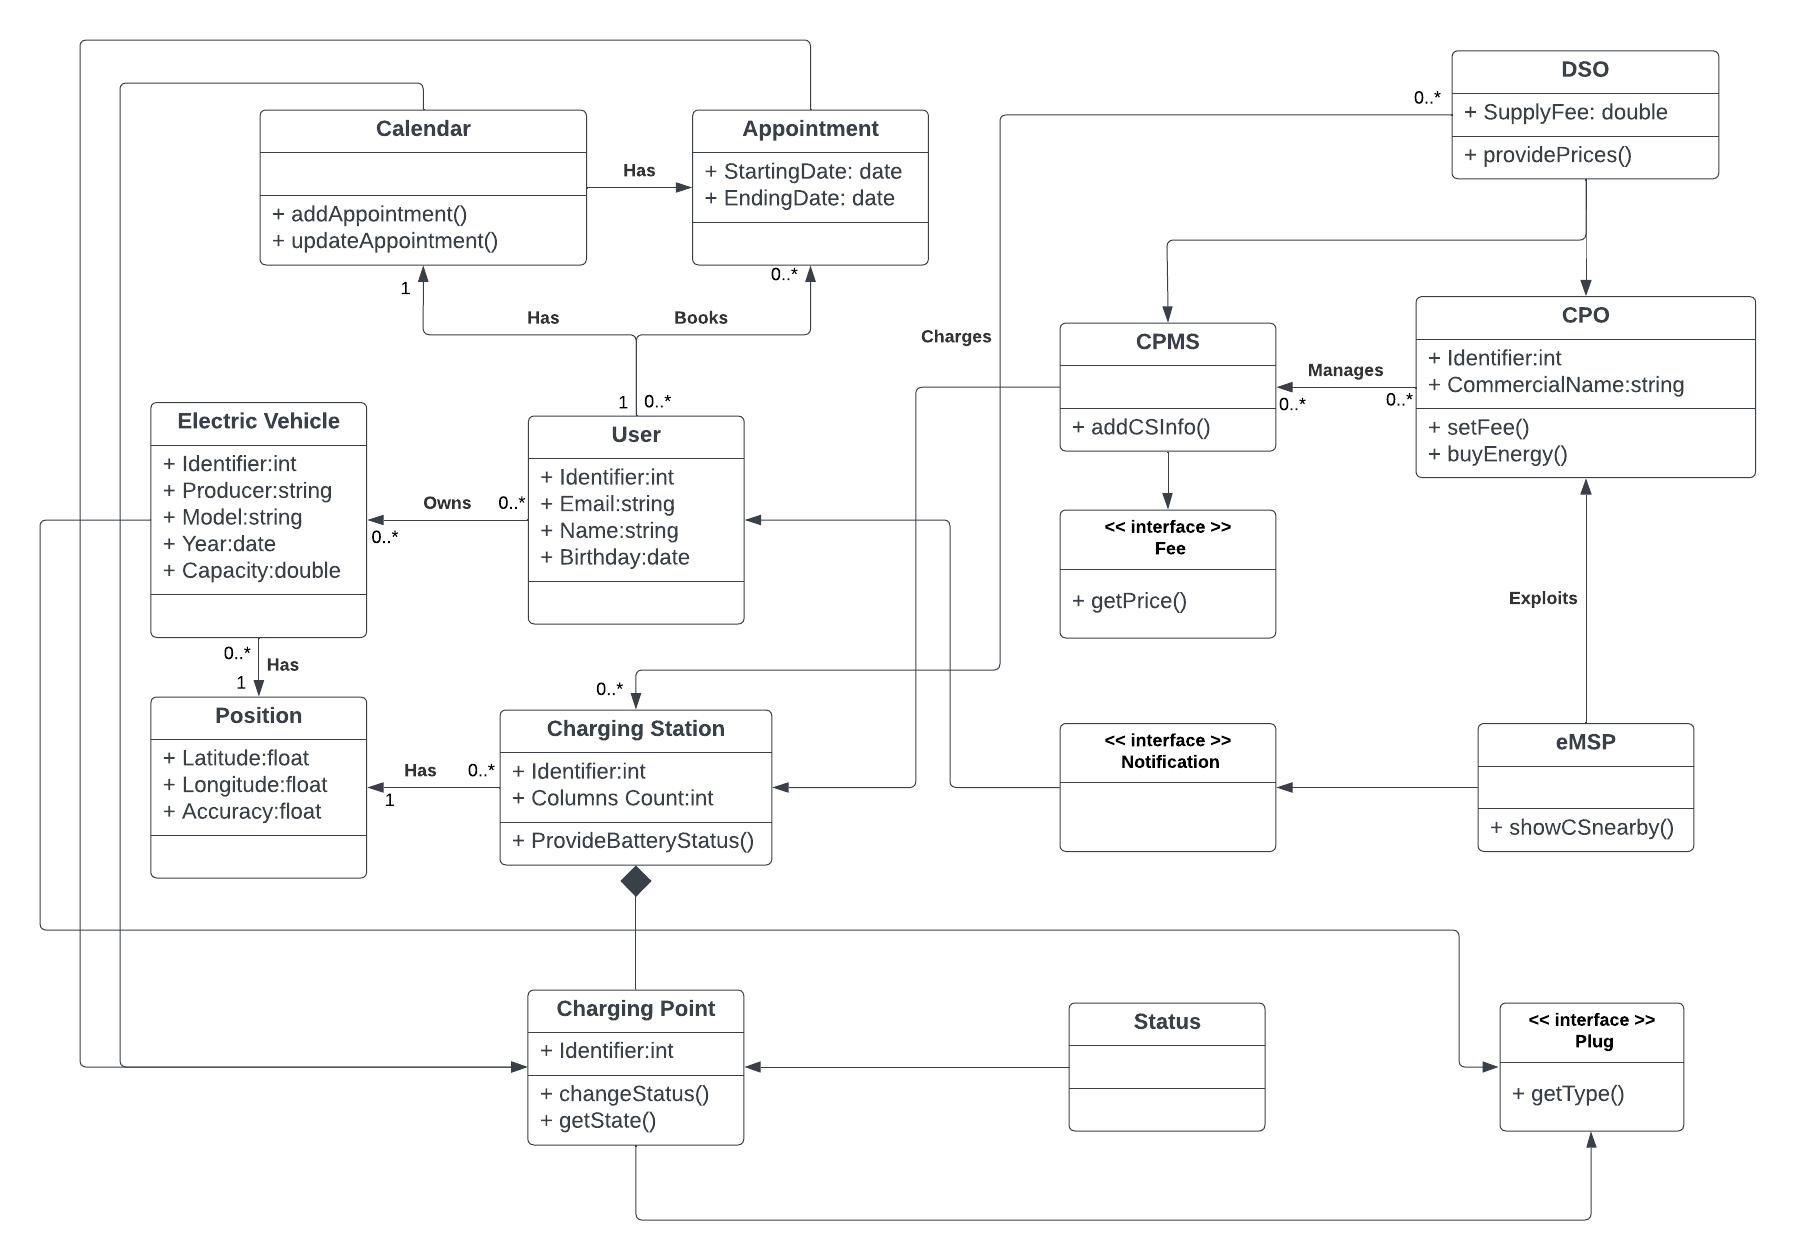
\includegraphics[width=0.9\linewidth]{ClassDiagrams/Class_Diagram_-_noPatterns}
        \caption{A simplified Class Diagram}
        \label{fig:class_diagram}%
    \end{center}
\end{figure}

\subsection{State Diagrams}
\label{subsec:state_diagrams}%

\paragraph{The EVD gets position and characteristics of charging stations at a certain location.}
EVD Andrew is going to use his car to go to the university for the Software Engineering 2 exam, but his EV is out of battery.
So, he needs to decide where to charge his vehicle.
To do that, he opens the \verb|eMALL| application and enters the map section.
At first, he sees if there is any charging station around him, but unfortunately at his current position,
there is only one charging station, which is shown as in maintenance.
So, he decides to see where to charge his EV nearby the university, inserting Milan in the location search bar.
From the huge amount of charging stations, he decides to choose the cheapest one.
He selects a charging station and gets its additional information.
He goes on searching other stations until he finds the best one for him.
At this point, the navigation process ends.

Below is presented a state diagram summarizing the flow of activities done in the charging stations navigation process:
\begin{figure}[H]
    \begin{center}
        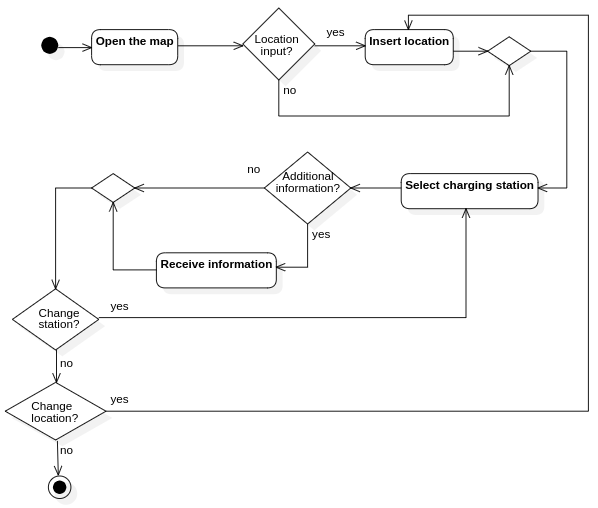
\includegraphics[width=0.8\linewidth]{StateDiagrams/get_charging_stations_location_state_diagram}
        \caption{Get locations of charging stations state diagram}
        \label{fig:locations_sd}%
    \end{center}
\end{figure}

\paragraph{EVD books a charge at a specified charging station at a certain timeframe.}
Andrew needs to book a charge for his EV\@.
He selects a charging station on the map and enters the booking section.
Unfortunately, the charging station cannot offer a reservation to him because no spots are available.
So, he searches for another one until he finds it.
Andrew has to decide in which timeframe he wants the charging point to be reserved.
So, he checks the availability schedule of the charging station and books a slot for its charge.
The system asks to pay a deposit to the EVD, which proceed to pay.
Finally, the EVD receives an e-mail with all the information that confirms the reservation.

It is shown a state diagram that summaries the activities in the booking process:
\begin{figure}[H]
    \begin{center}
        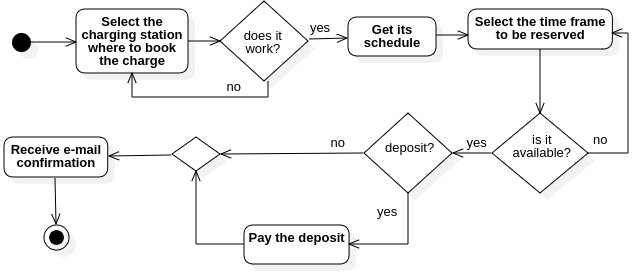
\includegraphics[width=0.9\linewidth]{StateDiagrams/book_a_charge_state_diagram}
        \caption{Book a charge state diagram}
        \label{fig:booking_sd}%
    \end{center}
\end{figure}

\paragraph{CPO adds charging points in its CPMS.}
\verb|SOLARIS| is the new company of the successful businessman Hugh Peter.
They decided to trust the \verb|eMALL| project, entrusting them with the responsibility of managing their IT infrastructure.
After logging in, they start inserting new charging points owned by them and distributed throughout the territory.
The first thing they are asked to select is the charging station to which the new spot belongs.
So, they insert all the requested information (serial number, location, connectors, power, etc.).
After they confirm and submit what they inserted, they iterate the process until they have inserted all the charging points.
It is shown a state diagram to summaries the activities in the charging points insertion process:
\begin{figure}[H]
    \begin{center}
        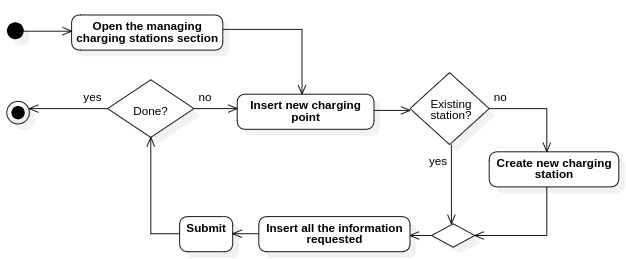
\includegraphics[width=0.9\linewidth]{StateDiagrams/insert_charging_points_state_diagram}
        \caption{Insert charging points state diagram}
        \label{fig:insert_charging_points_sd}%
    \end{center}
\end{figure}

\subsection{Scenarios}
\label{subsec:scenarios}%

\paragraph{Unregistered EVD creates an account.}
Mr. Oak has his EV and is looking for an application that offers the chance to charge his vehicle and smartly plan a
charging process depending on the battery status and his daily schedule.
Fortunately, he finds out \verb|eMALL|\@.
So, he immediately proceeds to create an account.
At first, he opens the application and goes to the ``sign up'' section.
The system asks to Mr. Oak if "he/she's a boy or a girl", in addition to personal information such as first and second name, birthday, living address, e-mail address, password, and telephone number, which he inserts immediately.
He receives an e-mail with a 6-digit code to be inserted in the new window shown by the \verb|eMALL| system to confirm his e-mail address.
After accepting the terms \& conditions and submitting all the inserted information, the system creates his account,
and he can begin using the application.

\paragraph{The EVD charges his/her EV.}
After booking a charge, Michael Scarn goes to the charging station at the chosen hour.
After turning off the EV, he opens the \verb|eMALL| application and enters the charge section.
From the set of close charging points, he selects which one has the serial number he received by \verb|eMALL| by e-mail
when he booked the charge.
So, he asks to charge the EV at that charging point.
After verifying that the EVD can be charged at that charging point, the application notifies to the user that the
connectors are now unlocked and ready to be used.\@
While the EV is in charge, the system notifies the EVD of the current status of the charging process.
When the process ends, he unplugs the connector, pays through the \verb|eMALL| application, and gets back in his car.

\paragraph{The EVD inserts a new activity in its calendar and receives a suggestion for a charging process.}
Jimothy inserts a new activity in his calendar, specifying the hour and destination of the event.
After doing that, he receives a notification that shows the EVD where and when to charge his vehicle.
The system creates suggestions to minimize the cost and the time lost at the charging station.
It also considers special offers activated by the CPOs registered in the eMALL system.
So, Joe accepts the received proposal and confirms the book of the listed charging points, making the needed payments.

\paragraph{The EVD receives a notification about a new special offer activated by a CPO}
Joe receives a notification about a new special offer activated by the CPO \verb|SOLARIS|.
So, he opens the promotion page, reads what it is about, and gets the discount code of the offer.
It consists of a 20\% discount for all the EVDs that are under 25.
Considering that he has to charge his EV, he decides to book a charging session at a charging station owned by the CPO \verb|SOLARIS|.
After selecting the timeframe and verifying its availability, he inserts the discount code SARTORIUS\@.


\section{Product functions}
\label{sec:product_functions}%
\textbf{The EVD books a charging session} \\
The main functionality of \verb|eMALL| is to book charge sessions in different charging stations for the EVD\@.
In particular, the system shows charging stations to the EVD and waits for him to select where he wants to book a charging session.

When \verb|eMALL| retrieves information about the charging stations available in the local area, it also retrieves all the extra info about the available plugs and power supplies.

The system has to control if the charging station is currently unavailable, and if it is not, it gets the station's schedule.
The EVD has to choose a timeframe between the ones available to book a charge session.
\verb|eMALL| also queries the charging station to know if the station has or not a mandatory deposit to pay to end the booking process.
If the station does not have a deposit policy, then \verb|eMALL| finishes the booking process by sending an informative email to the EVD that resumes all the booking info.

In the email, \verb|eMALL| also specifies the serial number associated with the charging point of the charging station where the EVD has to charge his EV\@.

\textbf{The EVD receives charging alerts about where to charge his EV} \\
\verb|eMALL| offers smart functions about when the EVD might book a charge for his EV\@.
Hence, when an EVD inserts a new activity in his calendar, \verb|eMALL| computes the best route to reach the destination through an external navigator API\@.
\verb|eMALL| also checks the battery status of the EV, so it notifies the best itinerary for the EVD\@.
If the battery state doesn't allow the EVD to reach the destination, then \verb|eMALL| shows him the best route with the charging stations available along the road.

\verb|eMALL| tries to minimize the costs.
Hence, starting from the current battery status, the system computes the maximum kilometers an EV can travel before running out of battery.
If the EV can reach the destination, \verb|eMALL| marks the route returned by the API as preferred.
On the other hand, \verb|eMALL| finds charging stations along the road and selects the one with the minimum costs because it knows the details about the EV, for instance, the plug type.
The best charging station found is shown to the EVD, allowing him to decide whether to start a booking process.

If the EVD doesn't accept \verb|eMALL| solution, he can book another charging station along the road and start, as well, a booking process.

\textbf{The CPO manages its charging stations} \\
A CPO should be able to manage its charging stations and relative charging points.
In general, a CPO might have new charging stations to register in \verb|eMALL|, and, as well, it might have charging points too.
The system allows the CPO to register charging stations, by entering all the info about them, for instance, the position on the map and the number of charging points available.
Furthermore, the system allows the registration of also charging points by inserting info like the available plugs and the power supply of the charging process.

Just like the CPO inserts new information about its product, it can also delete charging points or charging stations from \verb|eMALL|\@.

The system also shows CPOs charging stations and relative charging points on the map.
This functionality is necessary because they might break down, so the CPO has to change their availability status (offline, under maintenance, online).


\section{User characteristics}
\label{sec:user_characteristics}%
The actors listed below are considered in the eMALL system
\begin{itemize}
    \item \textbf{CPO:} owns one or more charging stations, and manages bookings and promotions about its charging points.
    He buys energy from DSOs, based on prices and needs.
    CPOs has their own IT system.
    \item \textbf{Unregistered EV Driver:} anybody who owns an electric vehicle, but isn’t registered in the eMALL system.
    Before accessing its benefits, it needs to get an account.
    \item \textbf{Registered EV Driver:} an electric vehicle owner who already joined the eMALL system, and access its benefits.
    He’s identified with a unique ID, and can own one or more vehicles with different specifics.
    They can check prices and position of charging points, in addition to receiving notifications about promotions reserved to them.
\end{itemize}


\section{Assumptions, dependencies and constraints}
\label{sec:assumptions_dependencies_and_constraints}%
\newcounter{da}
\setcounter{da}{1}
\newcommand{\cda}{\theda\stepcounter{da}}
\begin{center}
    \begin{longtable}{ |l|p{0.9\linewidth}| }
        \hline
        \textbf{ID} & \textbf{Description}                                                                                     \\
        \hline
        DA\cda      & Each user has needed competences to use the \verb|eMALL| system.                                         \\
        \hline
        DA\cda      & Both the users EVDs and CPOs have an e-mail.                                                             \\
        \hline
        DA\cda      & The EVD has a payment method.                                                                            \\
        \hline
        DA\cda      & The EVD uses a device with internet connectivity.                                                        \\
        \hline
        DA\cda      & The EVD uses a device with GPS module for navigation and localization.                                   \\
        \hline
        DA\cda      & There is a specific compatibility between EV's plug and connectors offered by charging points.           \\
        \hline
        DA\cda      & Charging points have their own software.                                                                 \\
        \hline
        DA\cda      & Communication between the \verb|eMALL| system and the charging points happens through the OCPP protocol. \\
        \hline
        DA\cda      & The \verb|eMALL| system communicates with EV brands API to get vehicles' specification.                  \\
        \hline
        DA\cda      & The \verb|eMALL| system communicates with DSOs through their APIs.                                       \\
        \hline
        DA\cda      & The \verb|eMALL| system communicates with third-party payment services to manage the payments.           \\
        \hline
        \caption{Domain assumptions.}
        \label{tab:domainassmptn_tab}%
    \end{longtable}
\end{center}



    \chapter{Specific Requirements}
    \label{ch:specific_requirements}%
    \section{External Interface Requirements}
\label{sec:external_interface_requirements}%

\subsection{User Interfaces}
\label{subsec:user_interfaces}%
The \verb|eMALL|’s user interfaces are a website and a mobile application;
the first is developed to be used mainly by CPOs with a dedicated login section for businesses but can be used by EVDs too.
The mobile application is available for Android and iOS and provides an enhanced experience as compared to the website
since it offers users personalized suggestions based on their location.
The website and the app should be easy to use since they will be used mostly by middle-aged users,
who might not always be familiar with the technology.
A “quick booking” section dedicated to facilitating the book process might be included,
for those EVDs who are used to booking a charge at the same charging station (based on suggestions given by AI).

\subsection{Hardware Interfaces}
\label{subsec:hardware_interfaces}%
The system only requires a smartphone or computer with an internet connection and web browser to access websites or mobile applications.
Furthermore, \verb|eMALL| communicates with the EV through its company's API to get the current battery level, the charging state,
so if it is plugged in and if it is charging, and the number of routable kilometers obtained on the current battery level.
To access personalized suggestions, based on EV’s position, the device in use has to be able to detect its location with a GPS localization system.

\subsection{Software Interfaces}
\label{subsec:software_interfaces}%
The following list describes the required software interfaces that the \verb|eMALL| system uses:
\begin{itemize}
    \item \textbf{CPMS and Charging Points.} The CPMS that is offered to the CPO communicates with the charging points
    through their API\@.
    Thanks to it, the system can manage the charging session, given the possibility of starting and stopping it or set
    the power supply to be given to each connected EV\@.
    Another significant functionality is the diagnostic of the charging point:
    a CPO can reboot its charging spots, can get their log, and can update their firmware.
    \item \textbf{eMALL and EVs.} The eMALL system communicates with the EVs registered by the EVD\@.
    As explained in the domain assumption section, we suppose that there is a third-party system that offers its API
    so to get the status of the battery of the EV\@.
    An example of a system that provides these features is Smartcar,
    which is already used by companies like AmpUp or BeCharge to remotely retrieve the battery level and remaining range of the EVs.
    \item \textbf{CPMS and DSOs.} The CPMSs offered to the CPO communicate with the DSOs through their APIs.
    CPOs can get selling prices set by the DSOs and they can decide from which DSO to acquire electricity.
    \item \textbf{eMALL and third-party payment services.} The \verb|eMALL| system offers the possibility to pay through
    external payment services to the EVD\@.
    The communication happens thanks to APIs offered by the companies that handle payments.
    \item \textbf{eMALL and Navigator Service.} The \verb|eMALL| system communicates with an external Navigator System to be able to map the position and compute paths between the provided location and the destination place.
\end{itemize}

\subsection{Communication Interfaces}
\label{subsec:communication_interfaces}%
The communication protocols that the \verb|eMALL| system uses are:
\begin{itemize}
    \item \textbf{Open Charge Point Protocol (OCPP).} It is used for the communication between the CPMS and the charging
    points.
    \item \textbf{HyperText Transfer Protocol over Secure Socket Layer (HTTPS).} The protocol is used every time data are
    exchanged with the external world.
    So, it is used when \verb|eMALL| communicates with EVDs and CPOs.
\end{itemize}


\section{Functional Requirements}
\label{sec:functional_requirements}%

\subsection{Requirements}
\label{subsec: requirements}%
The \verb|eMALL| system offers several functionalities to both EVDs and CPOs.
In the following table they are listed all the detected requirements that the system should respect in order to guarantee
the satisfiability of the goals:
\newpage
\newcounter{req}
\setcounter{req}{1}
\newcommand{\creq}{\thereq\stepcounter{req}}
\begin{center}
    \begin{longtable}{|l|p{0.9\linewidth}|}
        \hline
        \textbf{ID} & \textbf{Description}                                                                                                                             \\
        \hline
        R\creq      & The \verb|eMALL| system shall allow an unregistered EVD to create an account.                                                                    \\
        \hline
        R\creq      & The \verb|eMALL| system shall allow a registered EVD to log in.                                                                                  \\
        \hline
        R\creq      & The \verb|eMALL| system shall allow a registered EVD to add an EV in his profile.                                                                \\
        \hline
        R\creq      & The \verb|eMALL| system shall communicate with EV's brand API to get needed information.                                                         \\
        \hline
        R\creq      & The \verb|eMALL| system shall allow a registered EVD to book a charge.                                                                           \\
        \hline
        R\creq      & The \verb|eMALL| system shall allow a registered EVD to select a timeframe to reserve a charging point.                                          \\
        \hline
        R\creq      & The \verb|eMALL| system shall add a booked reservation into EVD's calendar.                                                                      \\
        \hline
        R\creq      & The \verb|eMALL| system shall allow a registered EVD to get all the charging station near to his current location.                               \\
        \hline
        R\creq      & The \verb|eMALL| system shall allow a registered EVD to insert a specific location to get charging station nearby.                               \\
        \hline
        R\creq      & The \verb|eMALL| system shall allow a registered EVD to move into the map of charging stations.                                                  \\
        \hline
        R\creq      & The \verb|eMALL| system shall allow a registered EVD to select a specific charging station.                                                      \\
        \hline
        R\creq      & The \verb|eMALL| system shall allow a registered EVD to get the location of a specific charging station.                                         \\
        \hline
        R\creq      & The \verb|eMALL| system shall allow a registered EVD to get the costs of a specific charging station.                                            \\
        \hline
        R\creq      & The \verb|eMALL| system shall allow a registered EVD to get the CPO owner of a specific charging station.                                        \\
        \hline
        R\creq      & The \verb|eMALL| system shall allow a registered EVD to get type of connectors of a specific charging station.                                   \\
        \hline
        R\creq      & The \verb|eMALL| system shall allow a registered EVD to get maximum power supply of the spots of a specific charging station.                    \\
        \hline
        R\creq      & The \verb|eMALL| system shall allow a registered EVD to get the status of a specific charging station.                                           \\
        \hline
        R\creq      & The \verb|eMALL| system shall allow a registered EVD to get the list of active promotions.                                                       \\
        \hline
        R\creq      & The \verb|eMALL| system shall allow a registered EVD to select a specific promotion.                                                             \\
        \hline
        R\creq      & The \verb|eMALL| system shall allow a registered EVD to activate a promotion.                                                                    \\
        \hline
        R\creq      & The \verb|eMALL| system shall allow a registered EVD to insert a new payment method.                                                             \\
        \hline
        R\creq      & The \verb|eMALL| system shall allow a registered EVD to select a payment method.                                                                 \\
        \hline
        R\creq      & The \verb|eMALL| system shall allow a registered EVD to pay with the preferred payment method.                                                   \\
        \hline
        R\creq      & The \verb|eMALL| system shall communicate with third-party payment services to make the payments.                                                \\
        \hline
        R\creq      & The \verb|eMALL| system shall allow a registered EVD to start a charging process.                                                                \\
        \hline
        R\creq      & The \verb|eMALL| system shall verify the identity of the EVD requesting to start a charging session.                                             \\
        \hline
        R\creq      & The \verb|eMALL| system shall communicate to charging points to unlock their plug.                                                               \\
        \hline
        R\creq      & The \verb|eMALL| system shall communicate to charging points to start the charging session.                                                      \\
        \hline
        R\creq      & The \verb|eMALL| system shall define the source of the charging session (batteries or DSO).                                                      \\
        \hline
        R\creq      & The \verb|eMALL| system shall define the power of the charging session.                                                                          \\
        \hline
        R\creq      & The \verb|eMALL| system shall get EV's battery status.                                                                                           \\
        \hline
        R\creq      & The \verb|eMALL| system shall send notifications about the current status of the charging session to the registered EVD.                         \\
        \hline
        R\creq      & The \verb|eMALL| system shall allow a registered EVD to stop the charging session.                                                               \\
        \hline
        R\creq      & The \verb|eMALL| system shall communicate to a charging point to stop the charging session.                                                      \\
        \hline
        R\creq      & The \verb|eMALL| system shall send the receipt of the charging session to the registered EVD.                                                    \\
        \hline
        R\creq      & The \verb|eMALL| system shall communicate the outcome of the payment to a registered EVD.                                                        \\
        \hline
        R\creq      & The \verb|eMALL| system shall allow a registered EVD to access in his own calendar.                                                              \\
        \hline
        R\creq      & The \verb|eMALL| system shall allow a registered EVD to add a new activity into his calendar.                                                    \\
        \hline
        R\creq      & The \verb|eMALL| system shall allow a registered EVD to specify the timeframe of a new activity.                                                 \\
        \hline
        R\creq      & The \verb|eMALL| system shall allow a registered EVD to specify the destination of a new activity.                                               \\
        \hline
        R\creq      & The \verb|eMALL| system shall save a new activity into EVD's calendar.                                                                           \\
        \hline
        R\creq      & The \verb|eMALL| system shall calculate the best schedules of where and when to charge registered EVD's EV so to minimize costs and wasted time. \\
        \hline
        R\creq      & The \verb|eMALL| system shall communicate to the registered EVD the details of the suggestions about the calculated schedules.                   \\
        \hline
        R\creq      & The \verb|eMALL| system shall allow a CPO to log in as a business user.                                                                          \\
        \hline
        R\creq      & The \verb|eMALL| system shall allow a CPO to manage its charging stations.                                                                       \\
        \hline
        R\creq      & The \verb|eMALL| system shall allow a CPO to set new selling prices for charging sessions.                                                       \\
        \hline
        R\creq      & The \verb|eMALL| system shall allow a CPO to add a new charging station in its profile.                                                          \\
        \hline
        R\creq      & The \verb|eMALL| system shall allow a CPO to specify the location of charging station (region, province, city, address).                         \\
        \hline
        R\creq      & The \verb|eMALL| system shall allow a CPO to specify the status of a charging station (available, maintenance, broken, unavailable).             \\
        \hline
        R\creq      & The \verb|eMALL| system shall allow a CPO to add a charging point in an existing charging station.                                               \\
        \hline
        R\creq      & The \verb|eMALL| system shall allow a CPO to specify the serial number of charging point.                                                        \\
        \hline
        R\creq      & The \verb|eMALL| system shall allow a CPO to specify the types of connectors of a charging point.                                                \\
        \hline
        R\creq      & The \verb|eMALL| system shall allow a CPO to specify the maximum power of a charging point.                                                      \\
        \hline
        R\creq      & The \verb|eMALL| system shall allow a CPO to specify the type of connectors of a charging point.                                                 \\
        \hline
        R\creq      & The \verb|eMALL| system shall reserve a charging point in a certain timeframe.                                                                   \\
        \hline
        R\creq      & The \verb|eMALL| system shall allow a CPO to manage its promotions.                                                                              \\
        \hline
        R\creq      & The \verb|eMALL| system shall allow a CPO to create a new promotion.                                                                             \\
        \hline
        R\creq      & The \verb|eMALL| system shall allow a CPO to specify the details of the a promotion.                                                             \\
        \hline
        R\creq      & The \verb|eMALL| system shall save the information of a promotion.                                                                               \\
        \hline
        R\creq      & The \verb|eMALL| system shall initialize the information of a new promotion.                                                                     \\
        \hline
        R\creq      & The \verb|eMALL| system shall allow a CPO to schedule a maintenance session for a charging station.                                              \\
        \hline
        R\creq      & The \verb|eMALL| system shall allow a CPO to specify date and starting hour of a maintenance session for a charging station.                     \\
        \hline
        R\creq      & The \verb|eMALL| system shall communicate to a charging station to schedule a maintenance at a specified timeframe.                              \\
        \hline
        R\creq      & The \verb|eMALL| system shall allow a CPO to get the list of DSOs.                                                                               \\
        \hline
        R\creq      & The \verb|eMALL| system shall allow a CPO to select a DSO from the list of DSOs.                                                                 \\
        \hline
        R\creq      & The \verb|eMALL| system shall allow a CPO to update its electricity provider.                                                                    \\
        \hline
        R\creq      & The \verb|eMALL| system shall communicate to a specified DSO to send energy to the charging stations of a CPO.                                   \\
        \hline
        R\creq      & The \verb|eMALL| system shall get the electricity selling prices from the DSOs.                                                                  \\
        \hline
        R\creq      & The \verb|eMALL| system shall store users information.                                                                                           \\
        \hline
        R\creq      & The \verb|eMALL| system shall allow the CPO to manage its company personal information.                                                          \\
        \hline
        \caption{Requirements.}
        \label{tab: req}%
    \end{longtable}
\end{center}

\subsection{Mapping on goals}
\label{subsec: map_on_g}%
In the following section it is shown how the relation $R\land D \models G$ holds.
In particular, at first it is shown a traceability matrix that associates domain assumptions and requirements to each goal.
After that, to facilitate reading, the section reports the text of all the assumptions and all the requirements related to each goal.
\newcounter{mg}
\setcounter{mg}{1}
\newcommand{\cmg}{\themg\stepcounter{mg}}
\begin{center}
    \begin{longtable}{|p{0.06\linewidth}|p{0.34\linewidth}|p{0.6\linewidth}|}
        \hline
        \textbf{Goal} & \textbf{Domain assumptions}                       & \textbf{Requirements}                                                               \\
        \hline
        G\cmg         & DA1, DA2, DA4, DA5                                & R1, R2, R8, R9, R10, R11, R12, R13, R14, R15, R16, R17, R69                         \\
        \hline
        G\cmg         & DA1, DA2, DA3, DA4, DA11                          & R1, R2, R18, R19, R20, R21, R22, R23, R24, R69                                      \\
        \hline
        G\cmg         & DA1, DA2, DA3, DA4, DA5, DA6, DA7, DA8, DA9, DA11 & R1, R2, R3, R4, R5, R6, R11, R21, R22, R23, R24, R69                                \\
        \hline
        G\cmg         & DA1, DA2, DA4, DA6, DA9                           & R1, R2, R4, R25, R26, R27, R28, R29, R30, R31, R32, R33, R35, R36, R69              \\
        \hline
        G\cmg         & DA1, DA2, DA4, DA5                                & R1, R2, R7, R37, R38, R39, R40, R41, R42, R43, R69                                  \\
        \hline
        G\cmg         & DA1, DA2, DA4                                     & R44, R45, R46, R47, R48, R49, R50, R51, R52, R53, R54, R55, R61, R62, R63, R69, R70 \\
        \hline
        G\cmg         & DA1, DA2, DA4, DA7, DA8, DA9                      & R4, R26, R27, R28, R29, R30, R31, R34, R44, R55, R69                                \\
        \hline
        G\cmg         & DA1, DA2, DA4                                     & R44, R56, R57, R58, R59, R60, R69                                                   \\
        \hline
        G\cmg         & DA1, DA2, DA4, DA9, DA10                          & R4, R44, R64, R65, R66, R67, R68, R69                                               \\
        \hline
        \caption{Mapping on goals.}
        \label{tab: map_on_g}%
    \end{longtable}
\end{center}

\subsubsection*{The EVD can get information about charging stations}
\begin{itemize}
    \item DA1. Each user has needed competences to use the \verb|eMALL| system.
    \item DA2. Both the users EVDs and CPOs have an e-mail..
    \item DA4. The EVD uses a device with internet connectivity.
    \item DA5. The EVD uses a device with GPS module for navigation and localization.
    \item R1. The \verb|eMALL| system shall allow an unregistered EVD to create an account.
    \item R2. The \verb|eMALL| system shall allow a registered EVD to log in.
    \item R8. The \verb|eMALL| system shall allow a registered EVD to get all the charging station
    near to his current location.
    \item R9. The \verb|eMALL| system shall allow a registered EVD to insert a specific location to
    get charging station nearby.
    \item R10.\ The \verb|eMALL| system shall allow a registered EVD to move into the map of charging
    stations.
    \item R11.\ The \verb|eMALL| system shall allow a registered EVD to select a specific charging
    station.
    \item R12.\ The \verb|eMALL| system shall allow a registered EVD to get the location of a specific
    charging station.
    \item R13.\ The \verb|eMALL| system shall allow a registered EVD to get the costs of a specific
    charging station.
    \item R14.\ The \verb|eMALL| system shall allow a registered EVD to get the CPO owner of a
    specific charging station.
    \item R15.\ The \verb|eMALL| system shall allow a registered EVD to get type of connectors of a
    specific charging station.
    \item R16.\ The \verb|eMALL| system shall allow a registered EVD to get maximum power supply
    of the spots of a specific charging station.
    \item R17.\ The \verb|eMALL| system shall allow a registered EVD to get the status of a specific
    charging station.
    \item R69.\ The \verb|eMALL| system shall store users information.
\end{itemize}

\subsubsection{The EVD can search for special offer provided by charging stations}
\begin{itemize}
    \item DA1. Each user has needed competences to use the \verb|eMALL| system.
    \item DA2. Both the users EVDs and CPOs have an e-mail..
    \item DA3. The EVD has a payment method.
    \item DA4. The EVD uses a device with internet connectivity.
    \item DA11.\ The \verb|eMALL| system communicates with third-party payment services to manage
    the payments.
    \item R1. The \verb|eMALL| system shall allow an unregistered EVD to create an account.
    \item R2. The \verb|eMALL| system shall allow a registered EVD to log in.
    \item R18.\ The \verb|eMALL| system shall allow a registered EVD to get the list of active promotions.
    \item R19.\ The \verb|eMALL| system shall allow a registered EVD to select a specific promotion.
    \item R20.\ The \verb|eMALL| system shall allow a registered EVD to activate a promotion.
    \item R21.\ The \verb|eMALL| system shall allow a registered EVD to insert a new payment method.
    \item R22.\ The \verb|eMALL| system shall allow a registered EVD to select a payment method.
    \item R23.\ The \verb|eMALL| system shall allow a registered EVD to pay with the preferred payment
    method.
    \item R24.\ The \verb|eMALL| system shall communicate with third-party payment services to make
    the payments.
    \item R69.\ The \verb|eMALL| system shall store users information.
\end{itemize}

\subsubsection{The EVD can book a charge for his EV at a charging station for a specified time frame}
\begin{itemize}
    \item DA1. Each user has needed competences to use the \verb|eMALL| system.
    \item DA2. Both the users EVDs and CPOs have an e-mail..
    \item DA3. The EVD has a payment method.
    \item DA4. The EVD uses a device with internet connectivity.
    \item DA5. The EVD uses a device with GPS module for navigation and localization.
    \item DA6. There is a specific compatibility between EV’s plug and connectors offered by
    charging points.
    \item DA7. Charging points have their own software.
    \item DA8. Communication between the \verb|eMALL| system and the charging points happens through the OCPP protocol.
    \item DA9. The \verb|eMALL| system communicates with EV brands API to get vehicles’ specification.
    \item DA11.\ The \verb|eMALL| system communicates with third-party payment services to manage
    the payments.
    \item R1. The \verb|eMALL| system shall allow an unregistered EVD to create an account.
    \item R2. The \verb|eMALL| system shall allow a registered EVD to log in.
    \item R3. The \verb|eMALL| system shall allow a registered EVD to add an EV in his profile.
    \item R4. The \verb|eMALL| system shall communicate with EV’s brand API to get needed information.
    \item R5. The \verb|eMALL| system shall allow a registered EVD to book a charge.
    \item R6. The \verb|eMALL| system shall allow a registered EVD to select a timeframe to reserve
    a charging point.
    \item R11.\ The \verb|eMALL| system shall allow a registered EVD to select a specific charging
    station.
    \item R21.\ The \verb|eMALL| system shall allow a registered EVD to insert a new payment method.
    \item R22.\ The \verb|eMALL| system shall allow a registered EVD to select a payment method.
    \item R23.\ The \verb|eMALL| system shall allow a registered EVD to pay with the preferred payment
    method.
    \item R24.\ The \verb|eMALL| system shall communicate with third-party payment services to make
    the payments.
    \item R69.\ The \verb|eMALL| system shall store users information.
\end{itemize}

\subsubsection{The EVD can charge his EV}
\begin{itemize}
    \item DA1. Each user has needed competences to use the \verb|eMALL| system.
    \item DA2. Both the users EVDs and CPOs have an e-mail..
    \item DA4. The EVD uses a device with internet connectivity.
    \item DA6. There is a specific compatibility between EV’s plug and connectors offered by
    charging points.
    \item DA9. The \verb|eMALL| system communicates with EV brands API to get vehicles’ specification.
    \item R1. The \verb|eMALL| system shall allow an unregistered EVD to create an account.
    \item R2. The \verb|eMALL| system shall allow a registered EVD to log in.
    \item R4. The \verb|eMALL| system shall communicate with EV’s brand API to get needed information.
    \item R25.\ The \verb|eMALL| system shall allow a registered EVD to start a charging process.
    \item R26.\ The \verb|eMALL| system shall verify the identity of the EVD requesting to start a
    charging session.
    \item R27.\ The \verb|eMALL| system shall communicate to charging points to unlock their plug.
    \item R28.\ The \verb|eMALL| system shall communicate to charging points to start the charging
    session.
    \item R29.\ The \verb|eMALL| system shall define the source of the charging session (batteries or
    DSO).
    \item R30.\ The \verb|eMALL| system shall define the power of the charging session.
    \item R31.\ The \verb|eMALL| system shall get EV’s battery status.
    \item R32.\ The \verb|eMALL| system shall send notifications about the current status of the charging
    session to the registered EVD\@.
    \item R33.\ The \verb|eMALL| system shall allow a registered EVD to stop the charging session.
    \item R35.\ The \verb|eMALL| system shall send the receipt of the charging session to the registered
    EVD\@.
    \item R36.\ The \verb|eMALL| system shall communicate the outcome of the payment to a registered
    EVD\@.
    \item R69.\ The \verb|eMALL| system shall store users information.
\end{itemize}

\subsubsection{The EVD can manage activities thanks to a calendar}
\begin{itemize}
    \item DA1. Each user has needed competences to use the \verb|eMALL| system.
    \item DA2. Both the users EVDs and CPOs have an e-mail..
    \item DA4. The EVD uses a device with internet connectivity.
    \item DA5. The EVD uses a device with GPS module for navigation and localization.
    \item R1. The \verb|eMALL| system shall allow an unregistered EVD to create an account.
    \item R2. The \verb|eMALL| system shall allow a registered EVD to log in.
    \item R7. The \verb|eMALL| system shall add a booked reservation into EVD’s calendar.
    \item R37.\ The \verb|eMALL| system shall allow a registered EVD to access in his own calendar.
    \item R38.\ The \verb|eMALL| system shall allow a registered EVD to add a new activity into his
    calendar.
    \item R39.\ The \verb|eMALL| system shall allow a registered EVD to specify the starting hour of a
    new activity.
    \item R40.\ The \verb|eMALL| system shall allow a registered EVD to specify the destination of a
    new activity.
    \item R41.\ The \verb|eMALL| system shall save a new activity into EVD’s calendar.
    \item R42.\ The \verb|eMALL| system shall calculate the best schedules of where and when to charge
    registered EVD’s EV so to minimize costs and wasted time.
    \item R43.\ The \verb|eMALL| system shall communicate to the registered EVD the details of the
    suggestions about the calculated schedules.
    \item R69.\ The \verb|eMALL| system shall store users information.
\end{itemize}

\subsubsection{The CPO can manage its charging stations and its charging points}
\begin{itemize}
    \item DA1. Each user has needed competences to use the \verb|eMALL| system.
    \item DA2. Both the users EVDs and CPOs have an e-mail..
    \item DA4. The EVD uses a device with internet connectivity.
    \item R44.\ The \verb|eMALL| system shall allow a CPO to log in as a business user.
    \item R45.\ The \verb|eMALL| system shall allow a CPO to manage its charging stations.
    \item R46.\ The \verb|eMALL| system shall allow a CPO to set new selling prices for charging sessions.
    \item R47.\ The \verb|eMALL| system shall allow a CPO to add a new charging station in its profile.
    \item R48.\ The \verb|eMALL| system shall allow a CPO to specify the location of charging station
    (region, province, city, address).
    \item R49.\ The \verb|eMALL| system shall allow a CPO to specify the status of a charging station
    (available, maintenance, broken, unavailable).
    \item R50.\ The \verb|eMALL| system shall allow a CPO to add a charging point in an existing
    charging station.
    \item R51.\ The \verb|eMALL| system shall allow a CPO to specify the serial number of charging
    point.
    \item R52.\ The \verb|eMALL| system shall allow a CPO to specify the types of connectors of a
    charging point.
    \item R53.\ The \verb|eMALL| system shall allow a CPO to specify the maximum power of a charging
    point.
    \item R54.\ The \verb|eMALL| system shall allow a CPO to specify the type of connectors of a
    charging point.
    \item R55.\ The \verb|eMALL| system shall reserve a charging point in a certain timeframe.
    \item R61.\ The \verb|eMALL| system shall allow a CPO to schedule a maintenance session for a
    charging station.
    \item R62.\ The \verb|eMALL| system shall allow a CPO to specify date and starting hour of a
    maintenance session for a charging station.
    \item R63.\ The \verb|eMALL| system shall communicate to a charging station to schedule a maintenance at a specified timeframe.
    \item R69.\ The \verb|eMALL| system shall store users information.
    \item R70.\ The \verb|eMALL| system shall allow the CPO to manage its company personal information.
\end{itemize}

\subsubsection{The CPO can manage a charging session}
\begin{itemize}
    \item DA1. Each user has needed competences to use the \verb|eMALL| system.
    \item DA2. Both the users EVDs and CPOs have an e-mail..
    \item DA4. The EVD uses a device with internet connectivity.
    \item DA7. Charging points have their own software.
    \item DA8. Communication between the \verb|eMALL| system and the charging points happens through the OCPP protocol.
    \item DA9. The \verb|eMALL| system communicates with EV brands API to get vehicles’ specification.
    \item R4. The \verb|eMALL| system shall communicate with EV’s brand API to get needed information.
    \item R26.\ The \verb|eMALL| system shall verify the identity of the EVD requesting to start a
    charging session.
    \item R27.\ The \verb|eMALL| system shall communicate to charging points to unlock their plug.
    \item R28.\ The \verb|eMALL| system shall communicate to charging points to start the charging
    session.
    \item R29.\ The \verb|eMALL| system shall define the source of the charging session (batteries or
    DSO).
    \item R30.\ The \verb|eMALL| system shall define the power of the charging session.
    \item R31.\ The \verb|eMALL| system shall get EV’s battery status.
    \item R34.\ The \verb|eMALL| system shall communicate to a charging point to stop the charging
    session.
    \item R44.\ The \verb|eMALL| system shall allow a CPO to log in as a business user.
    \item R55.\ The \verb|eMALL| system shall reserve a charging point in a certain timeframe.
    \item R69.\ The \verb|eMALL| system shall store users information.
\end{itemize}

\subsubsection{The CPO can manage its promotions}
\begin{itemize}
    \item DA1. Each user has needed competences to use the \verb|eMALL| system.
    \item DA2. Both the users EVDs and CPOs have an e-mail..
    \item DA4. The EVD uses a device with internet connectivity.
    \item R44.\ The \verb|eMALL| system shall allow a CPO to log in as a business user.
    \item R56.\ The \verb|eMALL| system shall allow a CPO to manage its promotions.
    \item R57.\ The \verb|eMALL| system shall allow a CPO to create a new promotion.
    \item R58.\ The \verb|eMALL| system shall allow a CPO to specify the details of the a promotion.
    \item R59.\ The \verb|eMALL| system shall save the information of a promotion.
    \item R60.\ The \verb|eMALL| system shall initialize the information of a new promotion.
    \item R69.\ The \verb|eMALL| system shall store users information.
\end{itemize}

\subsubsection{The CPO can manage the electricity supply}
\begin{itemize}
    \item DA1. Each user has needed competences to use the \verb|eMALL| system.
    \item DA2. Both the users EVDs and CPOs have an e-mail..
    \item DA4. The EVD uses a device with internet connectivity.
    \item DA9. The \verb|eMALL| system communicates with EV brands API to get vehicles’ specification.
    \item DA10.\ The \verb|eMALL| system communicates with DSOs through their APIs.
    \item R4. The \verb|eMALL| system shall communicate with EV’s brand API to get needed information.
    \item R44.\ The \verb|eMALL| system shall allow a CPO to log in as a business user.
    \item R64.\ The \verb|eMALL| system shall allow a CPO to get the list of DSOs.
    \item R65.\ The \verb|eMALL| system shall allow a CPO to select a DSO from the list of DSOs.
    \item R66.\ The \verb|eMALL| system shall allow a CPO to update its electricity provider.
    \item R67.\ The \verb|eMALL| system shall communicate to a specified DSO to send energy to the
    charging stations of a CPO\@.
    \item R68.\ The \verb|eMALL| system shall get the electricity selling prices from the DSOs.
    \item R69.\ The \verb|eMALL| system shall store users information.
\end{itemize}

\newpage

\subsection{Use case diagrams}
\label{subsec: use_case_diag}%
\subsubsection*{Unregistered EVD}
\begin{figure} [H]
    \begin{center}
        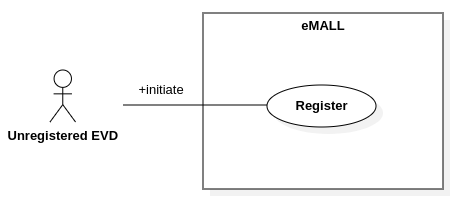
\includegraphics[width=0.7\linewidth]{Images/UseCaseDiagrams/unregistered_EVD_use_case_diagram}
        \caption{Unregistered EVD use case diagram.}
        \label{fig: unregistered_EVD_diag}
    \end{center}
\end{figure}

\subsubsection*{Registered EVD}
\begin{figure} [H]
    \begin{center}
        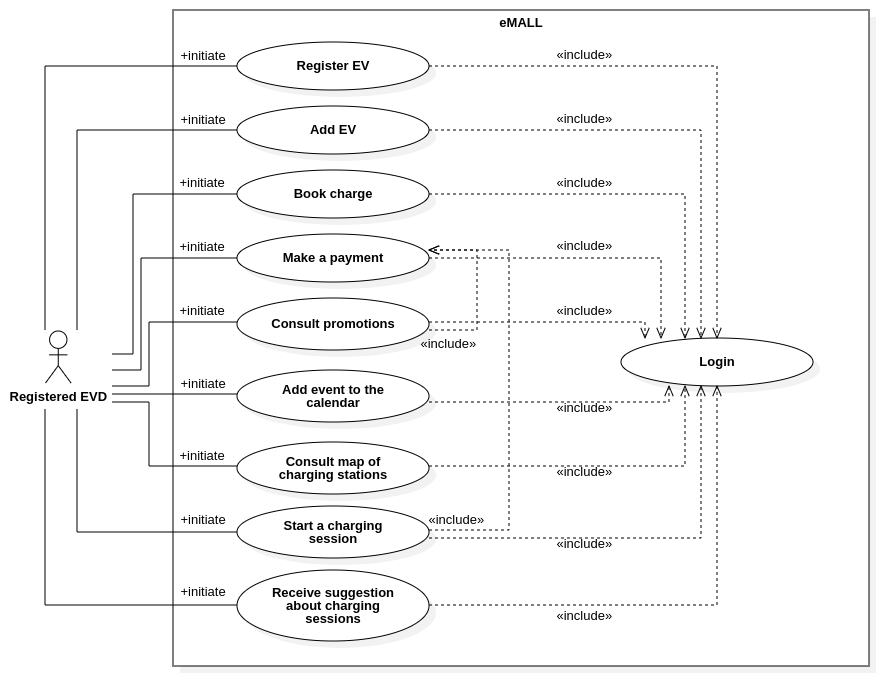
\includegraphics[width=0.9\linewidth]{Images/UseCaseDiagrams/registered_EVD_use_case_diagram}
        \caption{Unregistered EVD use case diagram.}
        \label{fig: reg_EVD_diag}
    \end{center}
\end{figure}

\subsubsection*{CPO}
\begin{figure} [H]
    \begin{center}
        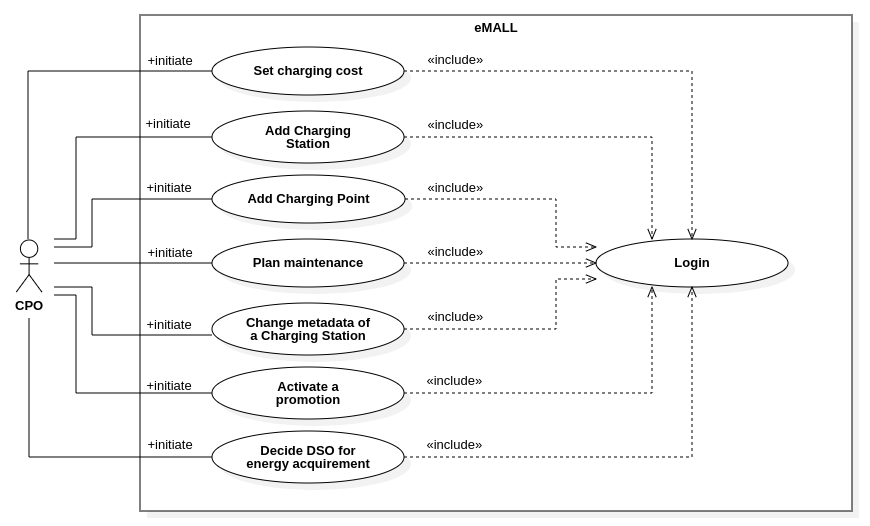
\includegraphics[width=0.9\linewidth]{Images/UseCaseDiagrams/CPO_use_case_diagram}
        \caption{Unregistered EVD use case diagram.}
        \label{fig: cpo_diag}
    \end{center}
\end{figure}

\subsection{Use cases}
\label{subsec: use_cases}%
\newcounter{uc}
\setcounter{uc}{1}
\newcommand{\cuc}{\theuc\stepcounter{uc}}
In this section, they are explained and represented the main identified use cases.
There is a table with entry conditions, event flow, exit conditions and exception for each of them, and a sequence diagram
that shows the messages exchanged between the entities and the called functions. \\
\subsubsection*{UC\cuc . EVD signs up}
\begin{center}
    \begin{longtable}{lp{0.75\linewidth}}
        \hline
        Actor            & Unregistered EVD                                                                                                                                                                                       \\
        \hline
        Entry conditions & The EVD isn’t registered in the \verb|eMALL| system, and he clicks the sign-up button                                                                                                                  \\
        \hline
        Event Flow       & 1.\ \verb|eMALL| asks the unregistered EVD to insert personal information (i.e., name, surname, birthday, billing address, e-mail, and password).                                                      \\
        & 2.\ The unregistered EVD fills out the form with his personal information (name, surname, birthday, billing address, e-mail, and password) and accepts the “Terms \& Conditions” and “Privacy Policy”. \\
        & 3.\ \verb|eMALL| validates the inserted EVD’s personal information.                                                                                                                                    \\
        & 4.\ \verb|eMALL| asks the unregistered EVD to insert payment method information.                                                                                                                       \\
        & 5.\ The EVD fills out a form with its payment method information.                                                                                                                                      \\
        & 6.\ \verb|eMALL| validates the inserted EVD’s payment method.                                                                                                                                          \\
        & 7.\ \verb|eMALL| sends a confirmation email to the EVD.                                                                                                                                                \\
        & 8.\ \verb|eMALL| sends back the EVD’s registration outcome.                                                                                                                                            \\
        \hline
        Exit condition   & An account is created.                                                                                                                                                                                 \\
        \hline
        Exceptions       & 3.1. \verb|eMALL| isn’t able to validate the EVD’s personal information.                                                                                                                               \\
        & 6.1. \verb|eMALL| isn’t able to validate the EVD’s payment method.                                                                                                                                     \\
        & In all these cases, the unregistered EVD is notified with an error message.                                                                                                                            \\
        \hline
        \caption{EVD signs up use case.}
        \label{tab: EVD_sign_up_use_case}
    \end{longtable}

    \begin{figure} [H]
        \begin{center}
            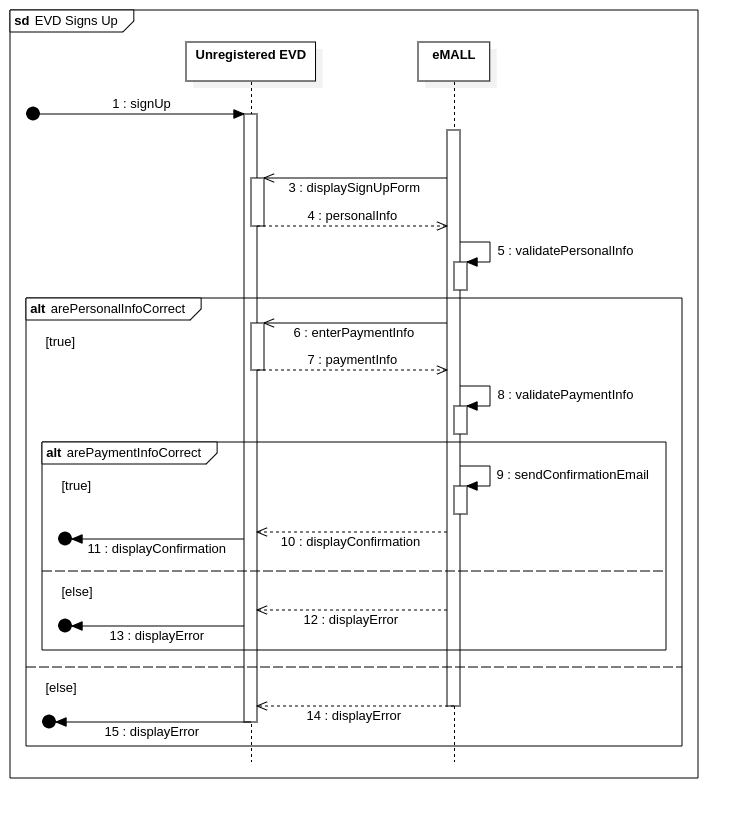
\includegraphics[width=0.9\linewidth]{Images/SequenceDiagrams/evd_signs_up}
            \caption{EVD signs up sequence diagram}
            \label{fig: evd_sign_up_seq_diag}
        \end{center}
    \end{figure}
\end{center}

\subsubsection*{UC\cuc . Registered EVD logs in}
\begin{center}
    \begin{longtable}{lp{0.75\linewidth}}
        \hline
        Actor            & Registered EVD                                                                              \\
        \hline
        Entry conditions & The EVD is registered in the \verb|eMALL| system and he clicks the log in button.           \\
        \hline
        Event Flow       & 1.\ \verb|eMALL| asks the registered EVD to insert the e-mail.                              \\
        & 2.\ The registered EVD inserts the e-mail.                                                  \\
        & 3.\ \verb|eMALL| validates the inserted e-mail.                                             \\
        & 4.\ \verb|eMALL| asks the registered EVD to insert the password associated with the e-mail. \\
        & 5.\ The registered EVD inserts the password.                                                \\
        & 6.\ \verb|eMALL| validates the inserted password in combination with the e-mail.            \\
        & 7.\ \verb|eMALL| sends back the login outcome.                                              \\
        \hline
        Exit condition   & The registered EVD access the \verb|eMALL| system.                                          \\
        \hline
        Exceptions       & 3.1 The e-mail is not recognized.                                                           \\
        & 6.1 The password is not correct.                                                            \\
        & In both cases, the registered EVD receives a notification through an error message.
        He has to insert his credentials again. \\
        \hline
        \caption{Registered EVD logs in use case.}
        \label{tab: EVD_logs_in_use_case}
    \end{longtable}


    \begin{figure} [H]
        \begin{center}
            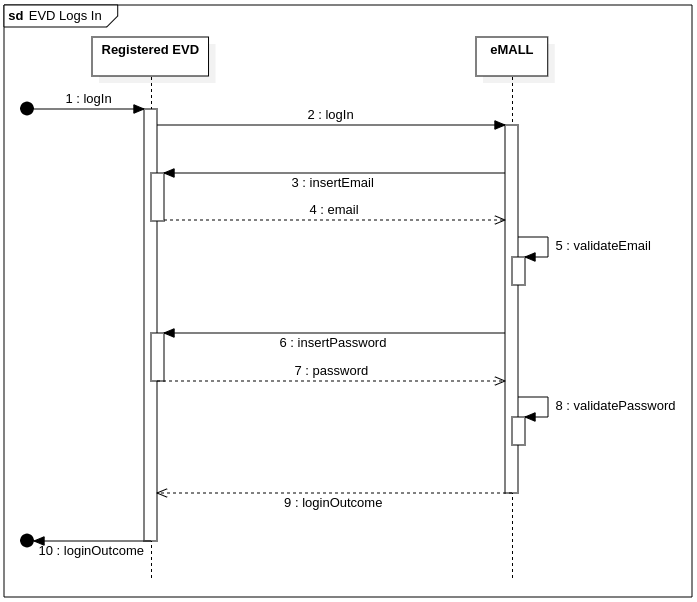
\includegraphics[width=0.9\linewidth]{Images/SequenceDiagrams/evd_logs_in}
            \caption{Registered EVD logs in sequence diagram}
            \label{fig: evd_logs_in_seq_diag}
        \end{center}
    \end{figure}
\end{center}

\newpage

\subsubsection*{UC\cuc . Registered EVD adds an EV}
\begin{center}
    \begin{longtable}{lp{0.75\linewidth}}
        \hline
        Actor            & Registered EVD                                                                                        \\
        \hline
        Entry conditions & The EVD is registered and correctly logged in.                                                        \\
        & The EVD clicks the ``Add a Vehicle'' button from his profile section of \verb|eMALL|                  \\
        \hline
        Event Flow       & 1.\ \verb|eMALL| asks the registered EVD to insert car information.                                   \\
        & 2.\ The registered EVD inserts the requested information and he sends them to the \verb|eMALL|.       \\
        & 3.\ \verb|eMALL| validates the information searching for possible errors.                             \\
        & 4.\ \verb|eMALL| asks the registered EVD to insert a nickname for the vehicle to save in his profile. \\
        & 5.\ The registered EVD inserts the nickname.                                                          \\
        & 6.\ \verb|eMALL| validates the nickname also searching for duplicates between user EV nicknames.      \\
        & 7.\ \verb|eMALL| sends back the registration outcome.                                                 \\
        \hline
        Exit condition   & Registered EVD correctly added a new EV in the profile.                                               \\
        \hline
        Exceptions       & 3.1 The e-mail is not recognized.                                                                     \\
        & 5.1 The inserted nickname is already taken between those owned by the user.                           \\
        & In both cases, the registered EVD receives a notification through an error message.                   \\
        \hline
        \caption{Registered EVD adds an EV use case.}
        \label{tab: EVD_adds_a_vehicle_use_case}
    \end{longtable}

    \begin{figure} [H]
        \begin{center}
            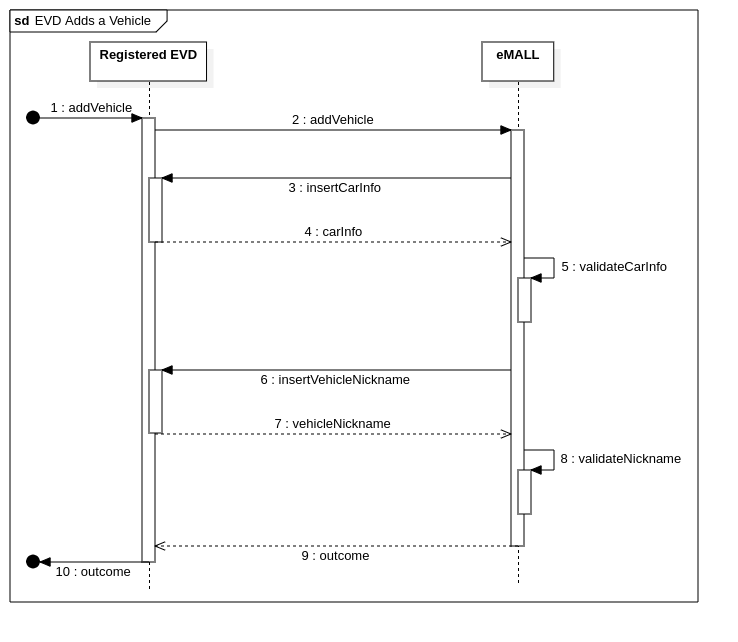
\includegraphics[width=0.9\linewidth]{Images/SequenceDiagrams/evd_adds_a_vehicle}
            \caption{Registered EVD adds an EV sequence diagram}
            \label{fig: evd_adds_ev_seq_diag}
        \end{center}
    \end{figure}
\end{center}

\subsubsection*{UC\cuc . Registered EVD books a charge}
\begin{center}
    \begin{longtable}{lp{0.75\linewidth}}
        \hline
        Actor            & Registered EVD                                                                                                \\
        \hline
        Entry conditions & The EVD is registered and correctly logged in.                                                                \\
        & The registered EVD selects a specific charging station and clicks the ``book'' button                         \\
        \hline
        Event Flow       & 1.\ \verb|eMALL| asks the registered EVD to choose a timeframe.                                               \\
        & 2.\ The registered EVD inserts the timeframe.                                                                 \\
        & 3.\ \verb|eMALL| checks if the selected timeframe is currently available.                                     \\
        & 4.\ \verb|eMALL| selects a charging point to reserve for the registered EVD depending on EV's specifications. \\
        & 5.\ \verb|eMALL| asks the registered EVD to confirm the booking with the prompted information.                \\
        & 6.\ The registered EVD clicks the ``Confirm'' button to confirm the booking.                                  \\
        & 7.\ \verb|eMALL| adds the booking to the registered EVD's calendar.                                           \\
        & 8.\ \verb|eMALL| sends back the booking outcome.                                                              \\
        \hline
        Exit condition   & A charging session is booked.                                                                                 \\
        \hline
        Exceptions       & 3.1. No free charging points are available at the selected timeframe.                                         \\
        & The registered EVD is notified with an error message, and asked to select a new timeframe.                    \\
        \hline
        \caption{Registered EVD books a charge use case.}
        \label{tab: EVD_booking_use_case}
    \end{longtable}

    \begin{figure} [H]
        \begin{center}
            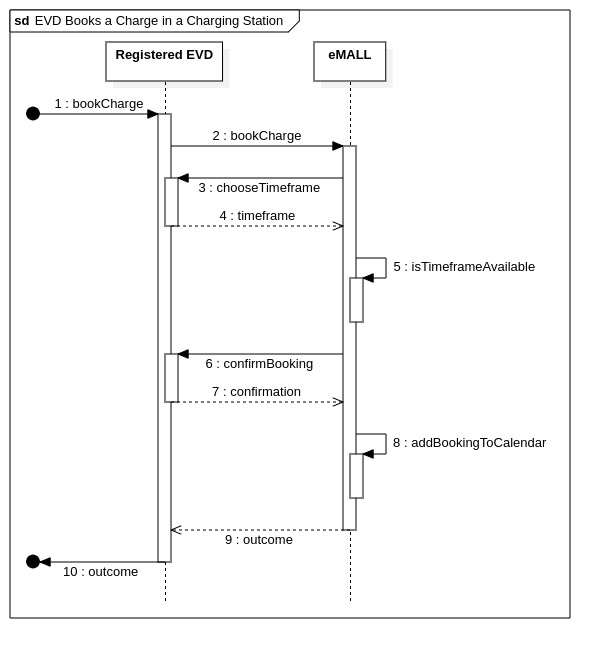
\includegraphics[width=0.9\linewidth]{Images/SequenceDiagrams/evd_books_a_charge_in_charging_station}
            \caption{Registered EVD books a charge sequence diagram}
            \label{fig: evd_books_charge_seq_diag}
        \end{center}
    \end{figure}
\end{center}

\newpage

\subsubsection*{UC\cuc . Registered EVD consults the map of charging stations}
\begin{center}
    \begin{longtable}{lp{0.75\linewidth}}
        \hline
        Actor            & Registered EVD                                                                                               \\
        \hline
        Entry conditions & The EVD is registered and correctly logged in.                                                               \\
        & The registered EVD is in the map section at a given or specified location.                                   \\
        \hline
        Event Flow       & 1.\ \verb|eMALL| shows the map with all the charging stations available over a specific location.            \\
        & 2.\ The registered EVD moves on the map, searching for a charging station.                                   \\
        & 3.\ \verb|eMALL| retrieves the charging station locations in the new place.                                  \\
        & 4.\ The registered EVD selects a specific charging station to get its detailed information.                  \\
        & 5.\ \verb|eMALL| retrieves the charging station's detailed information.                                      \\
        \hline
        Exit condition   & The registered EVD changes section, and moves from the dashboard.                                            \\
        \hline
        Exceptions       & 1.1 The registered EVD did not accept sharing location.                                                      \\
        & In this case, the registered EVD is notified by an error message and needs to move to its position manually. \\
        \hline
        \caption{Registered EVD consults the map of charging stations use case.}
        \label{tab: EVD_map_charging_stations_use_case}
    \end{longtable}

    \begin{figure} [H]
        \begin{center}
            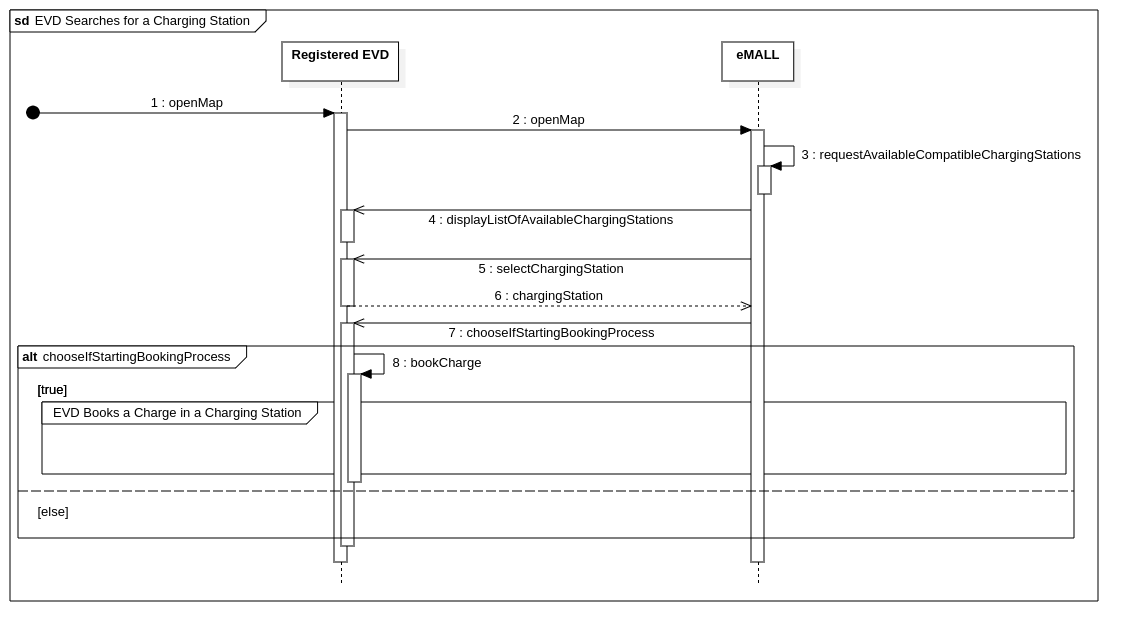
\includegraphics[width=0.9\linewidth]{Images/SequenceDiagrams/evd_searches_for_a_charging_station}
            \caption{Registered EVD consults the map of charging stations sequence diagram}
            \label{fig: evd_consults_stations_seq_diag}
        \end{center}
    \end{figure}
\end{center}

\subsubsection*{UC\cuc . Registered EVD consults a specific promotion that can be redeemed}
\begin{center}
    \begin{longtable}{lp{0.75\linewidth}}
        \hline
        Actor            & Registered EVD                                                                                                        \\
        \hline
        Entry conditions & The EVD is registered and correctly logged in.                                                                        \\
        & The EVD is in the promotion section.                                                                                  \\
        \hline
        Event Flow       & 1.\ \verb|eMALL| sends the promotion list to the registered EVD.                                                      \\
        & 2.\ The registered EVD selects a promotion to activate.                                                               \\
        & 3.\ The registered EVD triggers the offer.                                                                            \\
        & 4.\ \verb|eMALL| asks the registered EVD to choose between his payment methods.                                       \\
        & 5.\ The registered EVD picks the payment method.                                                                      \\
        & 6.\ \verb|eMALL| asks the registered EVD to confirm the payment.                                                      \\
        & 7.\ The registered EVD authorizes the payment.                                                                        \\
        & 8.\ \verb|eMALL| makes the payment.                                                                                   \\
        & 9.\ \verb|eMALL| sends back the payment outcome.                                                                      \\
        \hline
        Exit condition   & The promotion has been activated.                                                                                     \\
        \hline
        Exceptions       & 8.1. The payment fails due to no sufficient funds.                                                                    \\
        & 8.2. The payment fails due to the failure of the transaction.                                                         \\
        & 8.3. The payment fails because of data input errors.                                                                  \\
        & 8.4. The payment fails due to technical issues.                                                                       \\
        & In these cases, the registered EVD receives a notification with an error message, and the promotion is not activated. \\
        \hline
        \caption{Registered EVD consults a specific promotion that can be redeemed use case.}
        \label{tab: EVD_consults_promotion_use_case}
    \end{longtable}

    \begin{figure} [H]
        \begin{center}
            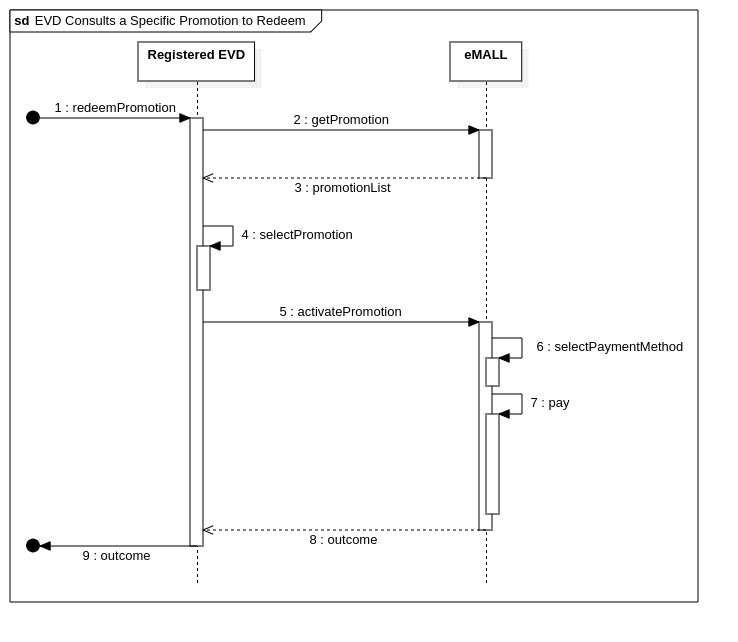
\includegraphics[width=0.9\linewidth]{Images/SequenceDiagrams/evd_consults_a_specific_promotion_to_redeem}
            \caption{Registered EVD consults a specific promotion that can be redeemed sequence diagram}
            \label{fig: evd_consults_promotion_seq_diag}
        \end{center}
    \end{figure}
\end{center}

\subsubsection*{UC\cuc . Registered EVD charges his EV}
\begin{center}
    \begin{longtable}{lp{0.75\linewidth}}
        \hline
        Actor            & Registered EVD                                                                                                              \\
        \hline
        Entry conditions & The EVD is registered and correctly logged in.                                                                              \\
        & The EVD asks the charging point to charge his EV.                                                                           \\
        \hline
        Event Flow       & 1.\ \verb|eMALL| communicates to the EVD if he has been correctly authenticated and if he can charge at the charging point. \\
        & 2.\ The registered EVD initializes the charging process.                                                                    \\
        & 3.\ \verb|eMALL| defines the source of the electricity (batteries or DSO).                                                  \\
        & 4.\ \verb|eMALL| defines how much electricity to give to the connected EV depending on actual energy demand.                \\
        & 5.\ \verb|eMALL| sends updates of the charging session to the EVD.                                                          \\
        & 6.\ The registered EVD stops the charging process.                                                                          \\
        & 7.\ \verb|eMALL| sends the receipt of the charging session to the EVD.                                                      \\
        & 8.\ The registered EVD makes the payment for the charging session.                                                          \\
        & 9.\ \verb|eMALL| sends back the payment outcome                                                                             \\
        \hline
        Exit condition   & The registered EVD has charged the EV and paid for the service received.                                                    \\
        \hline
        Exceptions       & 1.1 The registered EVD is not authorized to charge the EV at that charging point.                                           \\
        & 2.1 The EV is not correctly connected and the session can't be started.                                                     \\
        & In both cases, the registered EVD is notified with an error message.                                                        \\
        \hline
        \caption{Registered EVD charges his EV use case.}
        \label{tab: EVD_charges_EV_use_case}
    \end{longtable}
    \begin{figure} [H]
        \begin{center}
            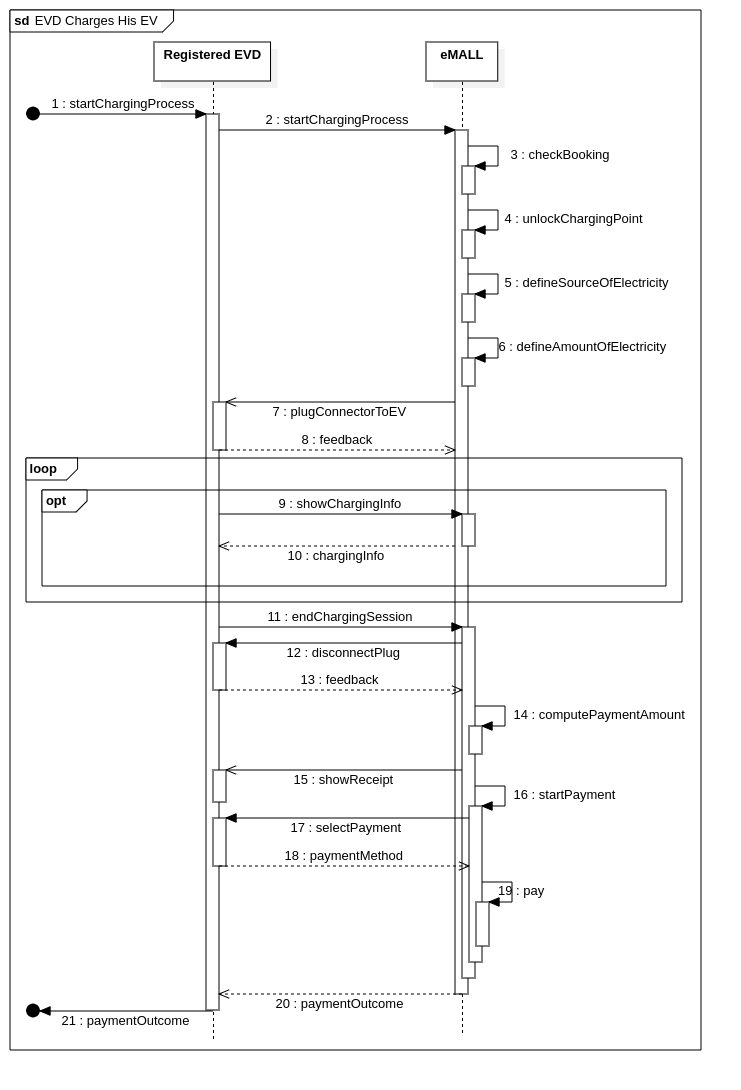
\includegraphics[width=0.9\linewidth]{Images/SequenceDiagrams/evd_charges_his_ev}
            \caption{Registered EVD charges his EV sequence diagram}
            \label{fig:evd_charges_ev_seq_diag}
        \end{center}
    \end{figure}
\end{center}

\subsubsection*{UC\cuc . Registered EVD makes a payment}
\begin{center}
    \begin{longtable}{lp{0.75\linewidth}}
        \hline
        Actor            & Registered EVD                                                                                                        \\
        \hline
        Entry conditions & The EVD is registered and correctly logged in.                                                                        \\
        & The registered EVD has decided the charging station where will charge the EV and is in the payment module.            \\
        \hline
        Event Flow       & 1.\ \verb|eMALL| shows registered EVD's payment methods and asks to select one of them.                               \\
        & 2.\ The registered EVD selects a payment method.                                                                      \\
        & 3.\ \verb|eMALL| verifies funds availability.                                                                         \\
        & 4.\ \verb|eMALL| starts the payment process.                                                                          \\
        & 5.\ \verb|eMALL| sends back the payment outcome.                                                                      \\
        \hline
        Exit condition   & The registered EVD has paid for a book or for a activation of a promotion.                                            \\
        \hline
        Exceptions       & 5.1. The payment fails due to no sufficient funds.                                                                    \\
        & 5.2. The payment fails due to the failure of the transaction.                                                         \\
        & 5.3. The payment fails because of data input errors.                                                                  \\
        & 5.4. The payment fails due to technical issues.                                                                       \\
        & In these cases, the registered EVD receives a notification with an error message, and the promotion is not activated. \\
        \hline
        \caption{Registered EVD makes a payment use case.}
        \label{tab: EVD_pays_use_case}
    \end{longtable}

    \begin{figure} [H]
        \begin{center}
            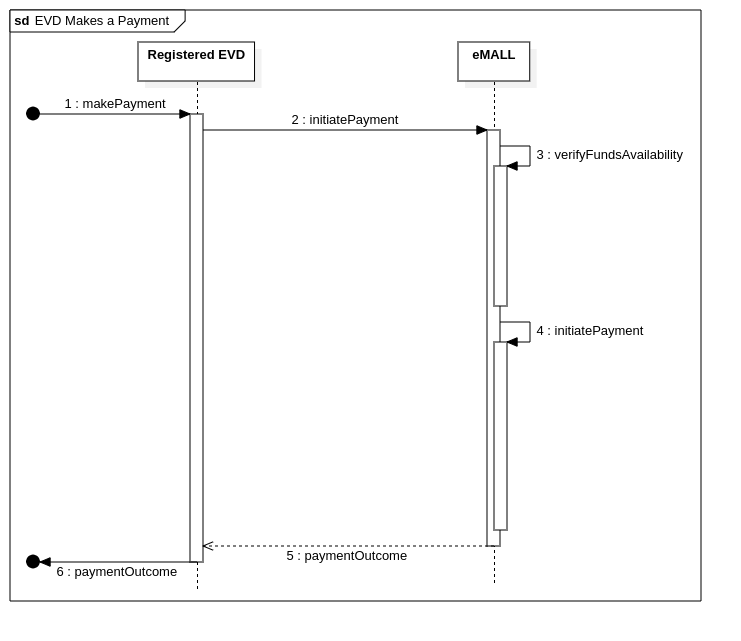
\includegraphics[width=0.9\linewidth]{Images/SequenceDiagrams/evd_makes_a_payment}
            \caption{Registered EVD makes a payment sequence diagram}
            \label{fig: evd_pays_seq_diag}
        \end{center}
    \end{figure}
\end{center}

\subsubsection*{UC\cuc . Registered EVD adds a new activity into the calendar and receives suggestions about charging schedule}
\begin{center}
    \begin{longtable}{lp{0.75\linewidth}}
        \hline
        Actor            & Registered EVD                                                                                                       \\
        \hline
        Entry conditions & The EVD is registered and correctly logged in.                                                                       \\
        & The registered EVD opens the calendar section.                                                                       \\
        \hline
        Event Flow       & 1.\ \verb|eMALL| shows the calendar to the registered EVD.                                                           \\
        & 2.\ The registered EVD clicks the ``insert new activity'' button.                                                    \\
        & 3.\ \verb|eMALL| sends the form to be compiled for the addition of a new activity.                                   \\
        & 4.\ The registered EVD inserts and submits the requested information.                                                \\
        & 5.\ \verb|eMALL| processes the received form.                                                                        \\
        & 6.\ \verb|eMALL| saves the new activity into registered EVD calendar.                                                \\
        & 7.\ \verb|eMALL| calculates the best schedule of where and when to charge the EV and sends it to the registered EVD. \\
        & 8.\ The registered EVD selects a charging station from the list of stations suggested by \verb|eMALL|.               \\
        & 9.\ \verb|eMALL| books the selected charging station at the specified timeframe.                                     \\
        & 10.\ \verb|eMALL| sends back the booking outcome to the registered EVD.                                              \\
        \hline
        Exit condition   & The registered EVD inserted a new activity received a suggestion about charging session.                             \\
        \hline
        Exceptions       & 5.1 The registered EVD has inserted a new activity that starts at the same hour of another one previously inserted.  \\
        & In this case, the registered EVD is notified with an error message and brought back to the calendar section.         \\
        \hline
        \caption{Registered EVD adds a new activity into the calendar and receives suggestions about charging schedule use case.}
        \label{tab: EVD_adds_activity_calendar_use_case}
    \end{longtable}

    \begin{figure} [H]
        \begin{center}
            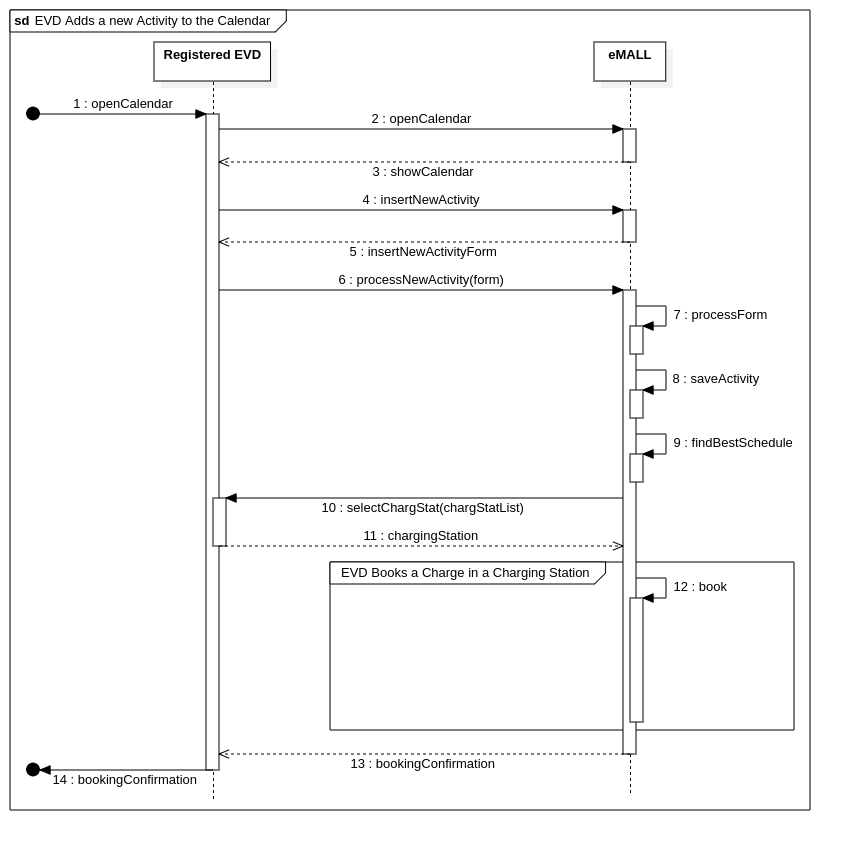
\includegraphics[width=0.8\linewidth]{Images/SequenceDiagrams/evd_adds_a_new_activity_to_the_calendar}
            \caption{Registered EVD adds a new activity into the calendar and receives suggestions about charging schedule sequence diagram}
            \label{fig: evd_adds_activity_seq_diag}
        \end{center}
    \end{figure}
\end{center}

\subsubsection*{UC\cuc . CPO logs in}
\begin{center}
    \begin{longtable}{lp{0.75\linewidth}}
        \hline
        Actor            & CPO                                                                                                 \\
        \hline
        Entry conditions & CPO’s operator is in the business login section.                                                    \\
        \hline
        Event Flow       & 1.\ \verb|eMALL| asks the CPO operator to insert his credentials to log in.                         \\
        & 2.\ The CPO operator inserts the CPO ID associated with its company, password, and email.           \\
        & 3.\ \verb|eMALL| validates the inserted credentials combination.                                    \\
        & 4.\ \verb|eMALL| sends back the login outcome.                                                      \\
        \hline
        Exit condition   & The CPO access the business section of the \verb|eMALL| system                                      \\
        \hline
        Exceptions       & 3.1.1. CPO credentials are not correct and not validated by \verb|eMALL|.                           \\
        & 3.2.1. CPO’s affiliate agreement has expired, and its ID is no longer allowed to access the system. \\
        & In both cases, the user receives a notification with an error message.                              \\
        & Also, in the second case, the operator is invited to call the sales team.                           \\
        \hline
        \caption{CPO logs in use case.}
        \label{tab: CPO_logs_in_use_case}
    \end{longtable}

    \begin{figure} [H]
        \begin{center}
            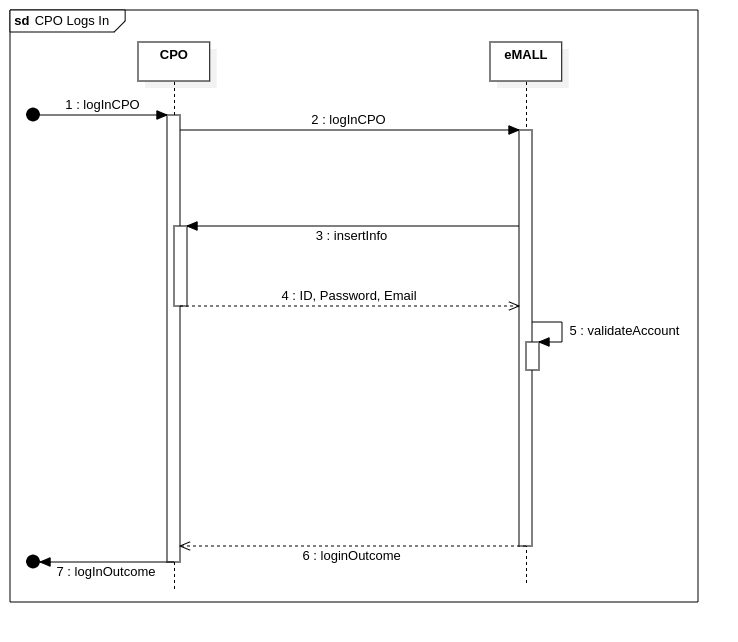
\includegraphics[width=0.9\linewidth]{Images/SequenceDiagrams/cpo_logs_in}
            \caption{CPO logs in sequence diagram}
            \label{fig: cpo_log_in_seq_diag}
        \end{center}
    \end{figure}
\end{center}

\subsubsection*{UC\cuc . CPO sets a fee}
\begin{center}
    \begin{longtable}{lp{0.75\linewidth}}
        \hline
        Actor            & CPO                                                                       \\
        \hline
        Entry conditions & The CPO is subscribed to the \verb|eMALL| system and correctly logged in. \\
        & The CPO enters the profile section.                                       \\
        \hline
        Event Flow       & 1.\ \verb|eMALL| shows the CPO his profile.                               \\
        & 2.\ The CPO enters the charging station managing section.                 \\
        & 3.\ \verb|eMALL| shows the CPO his managing charging station section.     \\
        & 4.\ The CPO taps the ``manage price'' button.                             \\
        & 5.\ The CPO inserts the value of the fee.                                 \\
        & 6.\ The CPO taps the submission button.                                   \\
        & 7.\ \verb|eMALL| sends back the outcome of the setting of the fee.        \\
        \hline
        Exit condition   & The fee is set to the new value.                                          \\
        \hline
        Exceptions       & 7.1 The CPO inserted a negative value.                                    \\
        & In this case, the system asks the CPO to insert a new value.              \\
        \hline
        \caption{CPO sets a fee use case.}
        \label{tab: CPO_sets_fee_use_case}
    \end{longtable}

    \begin{figure} [H]
        \begin{center}
            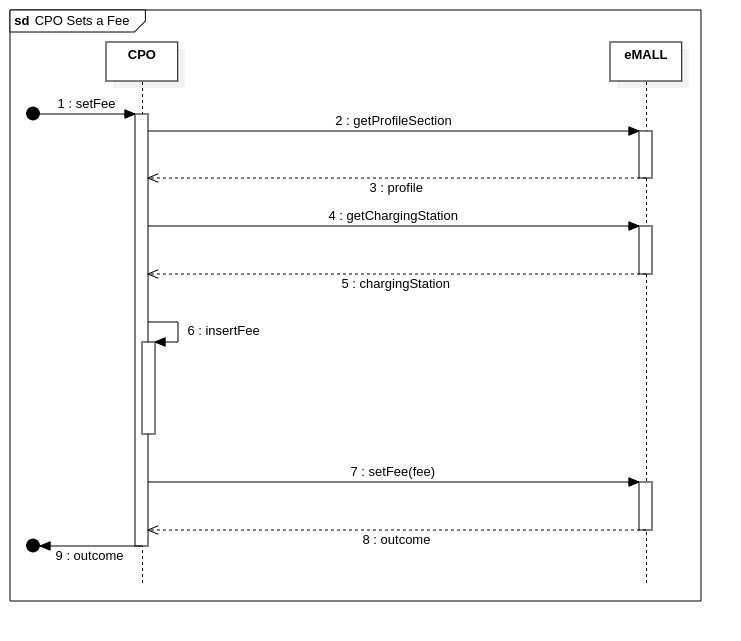
\includegraphics[width=0.9\linewidth]{Images/SequenceDiagrams/cpo_sets_a_fee}
            \caption{CPO sets a fee sequence diagram}
            \label{fig: cpo_sets_fee_seq_diag}
        \end{center}
    \end{figure}
\end{center}

\newpage

\subsubsection*{UC\cuc . CPO adds a charging station}
\begin{center}
    \begin{longtable}{lp{0.75\linewidth}}
        \hline
        Actor            & CPO                                                                                                       \\
        \hline
        Entry conditions & The CPO is subscribed to the \verb|eMALL| system and correctly logged in.                                 \\
        & The CPO is in the charging station section from the profile section.                                      \\
        & The CPO clicks the button to add a new charging station to its profile.                                   \\
        \hline
        Event Flow       & 1.\ \verb|eMALL| asks the CPO to insert the location of the new charging station.                         \\
        & 2.\ The CPO inserts the region, province, city, and address of the new charging station.                  \\
        & 3.\ \verb|eMALL| asks the CPO to insert the initial status of the new charging station.                   \\
        & 4.\ The CPO inserts the status of the new charging station (available, maintenance, broken, unavailable). \\
        & 5.\ \verb|eMALL| asks the CPO to insert the charging costs.                                               \\
        & 6.\ The CPO inserts the charging costs.                                                                   \\
        & 7.\ \verb|eMALL| asks the CPO to add charging points to the new charging station.                         \\
        & 8.\ The CPO inserts the information of the charging points.                                               \\
        & 9.\ \verb|eMALL| validates all the inserted information.                                                  \\
        & 10.\ \verb|eMALL| sends back the outcome of the insertion of the new charging station.                    \\
        \hline
        Exit condition   & The charging station is created and added to the CPO’s profile.                                           \\
        \hline
        Exceptions       & 9.1 There is already a charging station at the same location specified by the CPO.                        \\
        & The CPO receives a notification with an error message, and the charging station is not created.           \\
        \hline
        \caption{CPO adds a charging station use case.}
        \label{tab: CPO_adds_charging_station_use_case}
    \end{longtable}

    \begin{figure} [H]
        \begin{center}
            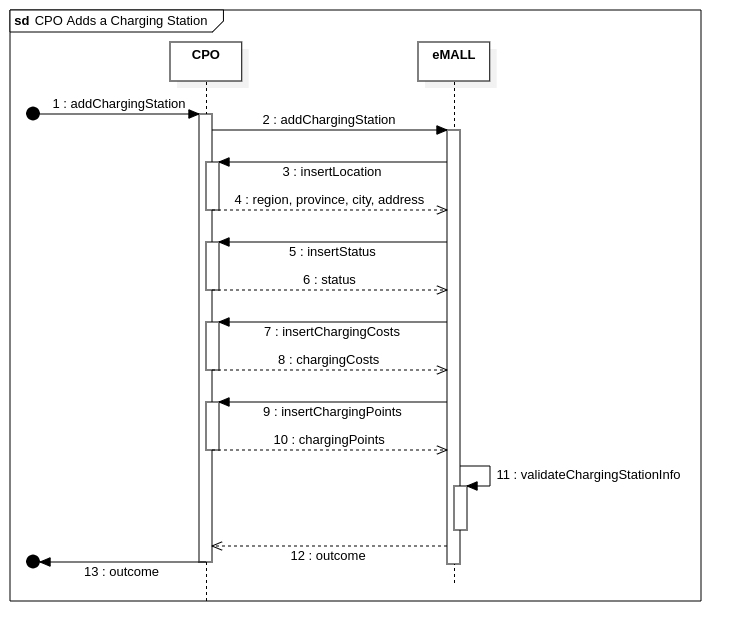
\includegraphics[width=0.9\linewidth]{Images/SequenceDiagrams/cpo_adds_a_charging_station}
            \caption{CPO adds a charging station sequence diagram}
            \label{fig: cpo_adds_station_seq_diag}
        \end{center}
    \end{figure}
\end{center}

\subsubsection*{UC\cuc . CPO adds a charging point}
\begin{center}
    \begin{longtable}{lp{0.75\linewidth}}
        \hline
        Actor            & CPO                                                                                             \\
        \hline
        Entry conditions & The CPO is subscribed to the \verb|eMALL| system and correctly logged in.                       \\
        & The CPO is in the charging station section from the profile section.                            \\
        & The CPO clicks the “add charging point” button.                                                 \\
        \hline
        Event Flow       & 1.\ \verb|eMALL| shows the CPO the list of its charging stations and asks it to select one.     \\
        & 2.\ The CPO selects a charging station.                                                         \\
        & 3.\ \verb|eMALL| asks the CPO to insert the information about the charging station.             \\
        & 4.\ The CPO inserts the serial number, the types of connectors installed on the charging point, the power supply,
        the initial status of the charging point, and the other required information. \\
        & 5.\ \verb|eMALL| validates the inserted information about the charging point.                   \\
        & 6.\ \verb|eMALL| sends back to the CPO the outcome of the creation of the new charging point.   \\
        \hline
        Exit condition   & The charging point is added to the charging station.                                            \\
        \hline
        Exceptions       & 4.1 There is already a charging point with the same serial number in the profile of the CPO.    \\
        & The CPO receives a notification with an error message, and the charging station is not created. \\
        \hline
        \caption{CPO adds a charging point use case.}
        \label{tab: CPO_adds_charging_point_use_case}
    \end{longtable}

    \begin{figure} [H]
        \begin{center}
            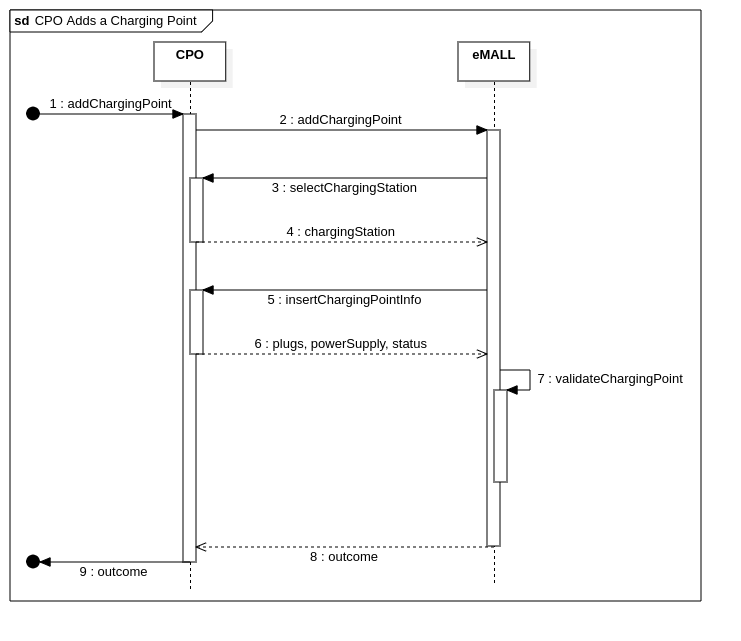
\includegraphics[width=0.9\linewidth]{Images/SequenceDiagrams/cpo_adds_a_charging_point}
            \caption{CPO adds a charging point sequence diagram}
            \label{fig: cpo_adds_point_seq_diag}
        \end{center}
    \end{figure}
\end{center}

\subsubsection*{UC\cuc . CPO changes the metadata of a charging point}
\begin{center}
    \begin{longtable}{lp{0.75\linewidth}}
        \hline
        Actor            & CPO                                                                                                     \\
        \hline
        Entry conditions & The CPO is subscribed to the \verb|eMALL| system and correctly logged in.                               \\
        & The CPO is in the charging station section from the profile section.                                    \\
        & The CPO clicks the “edit charging station” button.                                                      \\
        \hline
        Event Flow       & 1.\ \verb|eMALL| shows the CPO the list of its charging stations and asks it to select one.             \\
        & 2.\ The CPO selects a charging station.                                                                 \\
        & 3.\ \verb|eMALL| asks the CPO to insert the new values for the charging point.                          \\
        & 4.\ The CPO edits the metadata of the charging station.                                                 \\
        & 5.\ \verb|eMALL| updates the charging point with the new inserted values.                               \\
        & 6.\ \verb|eMALL| sends back to the CPO the outcome of the update.                                       \\
        \hline
        Exit condition   & The metadata of the charging station is updated.                                                        \\
        \hline
        Exceptions       & 4.1 The CPO inserts a new serial number of a charging point that is already registered into the system. \\
        & In this case, the system asks the CPO to insert again the value.                                        \\
        \hline
        \caption{CPO changes the metadata of a charging point use case.}
        \label{tab: CPO_updates_charging_point_use_case}
    \end{longtable}

    \begin{figure} [H]
        \begin{center}
            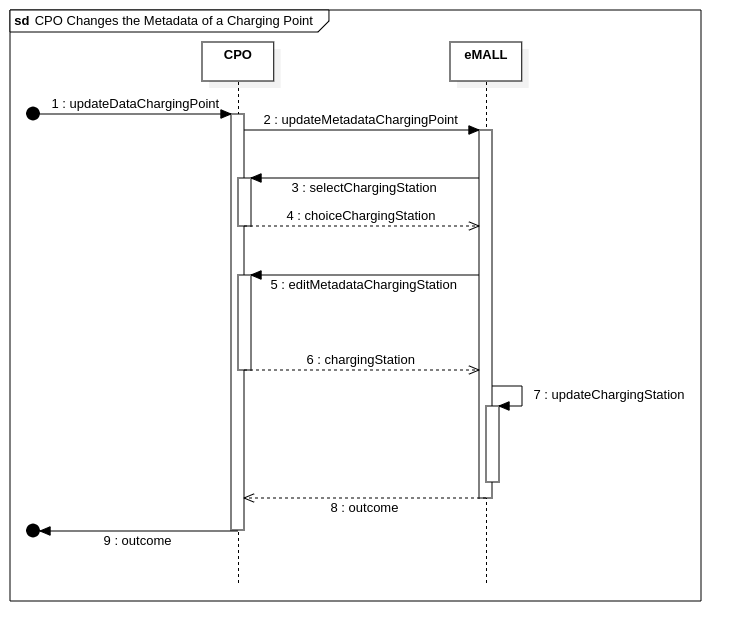
\includegraphics[width=0.9\linewidth]{Images/SequenceDiagrams/cpo_changes_the_metadata_of_a_charging_point}
            \caption{CPO changes the metadata of a charging point sequence diagram}
            \label{fig: cpo_updates_metadata_point_seq_diag}
        \end{center}
    \end{figure}
\end{center}

\subsubsection*{UC\cuc . CPO activates a promotion}
\begin{center}
    \begin{longtable}{lp{0.75\linewidth}}
        \hline
        Actor            & CPO                                                                                        \\
        \hline
        Entry conditions & The CPO is subscribed to the \verb|eMALL| system and correctly logged in.                  \\
        & The CPO is in the profile section.                                                         \\
        & The CPO clicks the “activate new promotion” button.                                        \\
        \hline
        Event Flow       & 1.\ \verb|eMALL| asks the CPO to define the features of the new promotion.                 \\
        & 2.\ The CPO defines the features of the new promotion.                                     \\
        & 3.\ \verb|eMALL| saves the new promotion.                                                  \\
        & 4.\ \verb|eMALL| initializes the promotion.                                                \\
        & 5.\ \verb|eMALL| sends back to the CPO the outcome of the activation of the new promotion. \\
        \hline
        Exit condition   & The promotion is created and activated.                                                    \\
        \hline
        Exceptions       & 2.1 The CPO inserted a date that is in the past.                                           \\
        & 2.2 The CPO inserted requirements of a promotion that conflict with its other promotions.  \\
        \hline
        \caption{CPO activates a promotion use case.}
        \label{tab: CPO_activates_promotion_use_case}
    \end{longtable}

    \begin{figure} [H]
        \begin{center}
            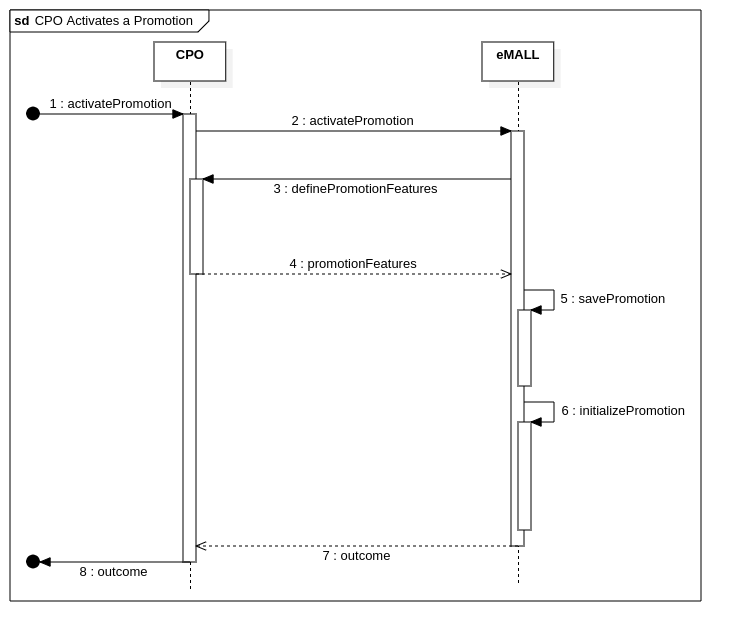
\includegraphics[width=0.9\linewidth]{Images/SequenceDiagrams/cpo_activates_a_promotion}
            \caption{CPO activates a promotion sequence diagram}
            \label{fig: cpo_activate_promo_seq_diag}
        \end{center}
    \end{figure}
\end{center}

\subsubsection*{UC\cuc . CPO plans a maintenance session for a charging station}
\begin{center}
    \begin{longtable}{lp{0.75\linewidth}}
        \hline
        Actor            & CPO                                                                                                            \\
        \hline
        Entry conditions & The CPO is subscribed to the \verb|eMALL| system and correctly logged in.                                      \\
        & The CPO is in the charging station section from the profile section and has selected a station.                \\
        & The CPO clicks the ``schedule maintenance'' button.                                                            \\
        \hline
        Event Flow       & 1.\ \verb|eMALL| asks the CPO to specify the date and the hour of the maintenance.                             \\
        & 2.\ \verb|eMALL| plans the maintenance session of the charging station.                                        \\
        & 3.\ \verb|eMALL| sends back the outcome of the planning of the maintenance to the CPO.                         \\
        \hline
        Exit condition   & It is planned a maintenance session for the specified charging station.                                        \\
        \hline
        Exceptions       & 2.1 The CPO tries to schedule a maintenance in a day that is in the past.                                      \\
        & 2.2 The CPO tries to schedule a maintenance that conflicts with another maintenance session already scheduled. \\
        \hline
        \caption{CPO plans a maintenance session for a charging station use case.}
        \label{tab: CPO_plans_maintenance_use_case}
    \end{longtable}
    \begin{figure} [H]
        \begin{center}
            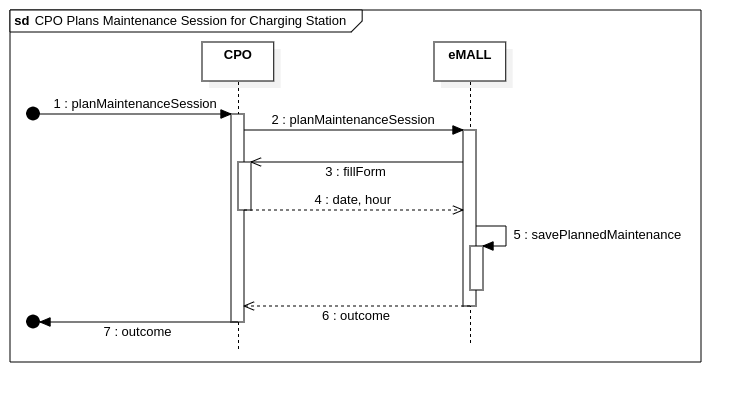
\includegraphics[width=0.9\linewidth]{Images/SequenceDiagrams/cpo_plans_maintenance_session_for_charging_station}
            \caption{CPO plans a maintenance session for a charging station sequence diagram}
            \label{fig: cpo_plans_maintenance_seq_diag}
        \end{center}
    \end{figure}
\end{center}

\subsubsection*{UC\cuc . CPO decides the DSO from which acquire energy}
\begin{center}
    \begin{longtable}{lp{0.75\linewidth}}
        \hline
        Actor            & CPO                                                                                                      \\
        \hline
        Entry conditions & The CPO is subscribed to the \verb|eMALL| system and correctly logged in.                                \\
        & The CPO is in the DSO section from the profile section.                                                  \\
        & The CPO clicks the “set DSO” button.                                                                     \\
        \hline
        Event Flow       & 1.\ \verb|eMALL| shows the CPO the list of DSOs.                                                         \\
        & 2.\ \verb|eMALL| asks the CPO to select a DSO from the list.                                             \\
        & 3.\ The CPO selects a DSO from the list.                                                                 \\
        & 4.\ \verb|eMALL| updates CPO’s profile information.                                                      \\
        & 5.\ \verb|eMALL| activates the selected DSO as the one from which to acquire energy.                     \\
        & 6.\ \verb|eMALL| sends back to the CPO the outcome of the setting of the DSO                             \\
        \hline
        Exit condition   & The DSO from which to acquire energy is updated.                                                         \\
        \hline
        Exceptions       & 3.1 It is impossible to communicate with the chosen DSO, so it can't be set as new electricity provider. \\
        & In this case, the CPO is asked to select another DSO or to end the process.                              \\
        \hline
        \caption{CPO decides the DSO from which acquire energy use case.}
        \label{tab: CPO_decides_DSO_use_case}
    \end{longtable}

    \begin{figure} [H]
        \begin{center}
            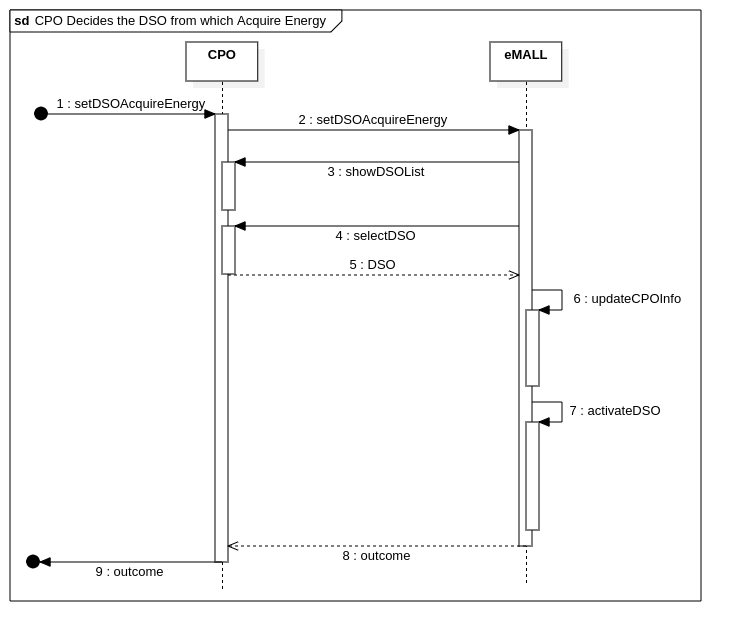
\includegraphics[width=0.9\linewidth]{Images/SequenceDiagrams/cpo_decides_the_dso_from_which_acquire_energy}
            \caption{CPO decides the DSO from which acquire energy sequence diagram}
            \label{fig: cpo_decides_DSO_seq_diag}
        \end{center}
    \end{figure}
\end{center}

\subsection{Mapping on requirements}
\label{subsec: map_on_req}%
\newcounter{mr}
\setcounter{mr}{1}
\newcommand{\cmr}{\themr\stepcounter{mr}}
\begin{center}
    \begin{longtable}{p{0.12\linewidth}p{0.88\linewidth}}
        \hline
        \textbf{Use Case} & \textbf{Requirements}                                                                                                                                  \\
        \hline
        UC\cmr            & R1. The \verb|eMALL| system shall allow an unregistered EVD to create an account.                                                                      \\
        & R21.\ The \verb|eMALL| system shall allow a registered EVD to insert a new payment method.                                                             \\
        & R24.\ The \verb|eMALL| system shall communicate with third-party payment services to make the payments.                                                \\
        & R69.\ The \verb|eMALL| system shall store users information.                                                                                           \\
        \hline
        UC\cmr            & R2. The \verb|eMALL| system shall allow a registered EVD to log in.                                                                                    \\
        \hline
        UC\cmr            & R2. The \verb|eMALL| system shall allow a registered EVD to log in.                                                                                    \\
        & R3. The \verb|eMALL| system shall allow a registered EVD to add an EV in his profile.                                                                  \\
        & R4. The \verb|eMALL| system shall communicate with EV’s brand API to get needed information.                                                           \\
        & R11.\ The \verb|eMALL| system shall allow a registered EVD to select a specific charging station.                                                      \\
        \hline
        UC\cmr            & R2. The \verb|eMALL| system shall allow a registered EVD to log in.                                                                                    \\
        & R5. The \verb|eMALL| system shall allow a registered EVD to book a charge.                                                                             \\
        & R6. The \verb|eMALL| system shall allow a registered EVD to select a timeframe to reserve a charging point.                                            \\
        & R7. The \verb|eMALL| system shall add a booked reservation into EVD’s calendar.                                                                        \\
        & R55.\ The \verb|eMALL| system shall reserve a charging point in a certain timeframe.                                                                   \\
        & R69.\ The \verb|eMALL| system shall store users information.                                                                                           \\
        \hline
        UC\cmr            & R2. The \verb|eMALL| system shall allow a registered EVD to log in.                                                                                    \\
        & R8. The \verb|eMALL| system shall allow a registered EVD to get all the charging station near to his current location.                                 \\
        & R9. The \verb|eMALL| system shall allow a registered EVD to insert a specific location to get charging station nearby.                                 \\
        & R10.\ The \verb|eMALL| system shall allow a registered EVD to move into the map of charging stations.                                                  \\
        & R11.\ The \verb|eMALL| system shall allow a registered EVD to select a specific charging station.                                                      \\
        & R12.\ The \verb|eMALL| system shall allow a registered EVD to get the location of a specific charging station.                                         \\
        & R13.\ The \verb|eMALL| system shall allow a registered EVD to get the costs of a specific charging station.                                            \\
        & R14.\ The \verb|eMALL| system shall allow a registered EVD to get the CPO owner of a specific charging station.                                        \\
        & R15.\ The \verb|eMALL| system shall allow a registered EVD to get type of connectors of a specific charging station.                                   \\
        & R16.\ The \verb|eMALL| system shall allow a registered EVD to get maximum power supply of the spots of a specific charging station.                    \\
        & R17.\ The \verb|eMALL| system shall allow a registered EVD to get the status of a specific charging station.                                           \\
        & R69.\ The \verb|eMALL| system shall store users information.                                                                                           \\
        \hline
        UC\cmr            & R2. The \verb|eMALL| system shall allow a registered EVD to log in.                                                                                    \\
        & R18.\ The \verb|eMALL| system shall allow a registered EVD to get the list of active promotions.                                                       \\
        & R19.\ The \verb|eMALL| system shall allow a registered EVD to select a specific promotion.                                                             \\
        & R20.\ The \verb|eMALL| system shall allow a registered EVD to activate a promotion.                                                                    \\
        & R21.\ The \verb|eMALL| system shall allow a registered EVD to insert a new payment method.                                                             \\
        & R22.\ The \verb|eMALL| system shall allow a registered EVD to select a payment method.                                                                 \\
        & R23.\ The \verb|eMALL| system shall allow a registered EVD to pay with the preferred payment method.                                                   \\
        & R24.\ The \verb|eMALL| system shall communicate with third-party payment services to make the payments.                                                \\
        & R69.\ The \verb|eMALL| system shall store users information.                                                                                           \\
        \hline
        UC\cmr            & R2. The \verb|eMALL| system shall allow a registered EVD to log in.                                                                                    \\
        & R22.\ The \verb|eMALL| system shall allow a registered EVD to select a payment method.                                                                 \\
        & R23.\ The \verb|eMALL| system shall allow a registered EVD to pay with the preferred payment method.                                                   \\
        & R24.\ The \verb|eMALL| system shall communicate with third-party payment services to make the payments.                                                \\
        & R25.\ The \verb|eMALL| system shall allow a registered EVD to start a charging process.                                                                \\
        & R26.\ The \verb|eMALL| system shall verify the identity of the EVD requesting to start a charging session.                                             \\
        & R27.\ The \verb|eMALL| system shall communicate to charging points to unlock their plug.                                                               \\
        & R28.\ The \verb|eMALL| system shall communicate to charging points to start the charging session.                                                      \\
        & R29.\ The \verb|eMALL| system shall define the source of the charging session (batteries or DSO).                                                      \\
        & R30.\ The \verb|eMALL| system shall define the power of the charging session.                                                                          \\
        & R31.\ The \verb|eMALL| system shall get EV’s battery status.                                                                                           \\
        & R32.\ The \verb|eMALL| system shall send notifications about the current status of the charging session to the registered EVD\@.                       \\
        & R33.\ The \verb|eMALL| system shall allow a registered EVD to stop the charging session.                                                               \\
        & R34.\ The \verb|eMALL| system shall communicate to a charging point to stop the charging session.                                                      \\
        & R35.\ The \verb|eMALL| system shall send the receipt of the charging session to the registered EVD\@.                                                  \\
        & R36.\ The \verb|eMALL| system shall communicate the outcome of the payment to a registered EVD\@.                                                      \\
        & R69.\ The \verb|eMALL| system shall store users information.                                                                                           \\
        \hline
        UC\cmr            & R2. The \verb|eMALL| system shall allow a registered EVD to log in.                                                                                    \\
        & R22.\ The \verb|eMALL| system shall allow a registered EVD to select a payment method.                                                                 \\
        & R23.\ The \verb|eMALL| system shall allow a registered EVD to pay with the preferred payment method.                                                   \\
        & R24.\ The \verb|eMALL| system shall communicate with third-party payment services to make the payments.                                                \\
        & R69.\ The \verb|eMALL| system shall store users information.                                                                                           \\
        \hline
        UC\cmr            & R2. The \verb|eMALL| system shall allow a registered EVD to log in.                                                                                    \\
        & R5. The \verb|eMALL| system shall allow a registered EVD to book a charge.                                                                             \\
        & R11.\ The \verb|eMALL| system shall allow a registered EVD to select a specific charging station.                                                      \\
        & R37.\ The \verb|eMALL| system shall allow a registered EVD to access in his own calendar.                                                              \\
        & R38.\ The \verb|eMALL| system shall allow a registered EVD to add a new activity into his calendar.                                                    \\
        & R39.\ The \verb|eMALL| system shall allow a registered EVD to specify the starting hour of a new activity.                                             \\
        & R40.\ The \verb|eMALL| system shall allow a registered EVD to specify the destination of a new activity.                                               \\
        & R41.\ The \verb|eMALL| system shall save a new activity into EVD’s calendar.                                                                           \\
        & R42.\ The \verb|eMALL| system shall calculate the best schedules of where and when to charge registered EVD’s EV so to minimize costs and wasted time. \\
        & R43.\ The \verb|eMALL| system shall communicate to the registered EVD the details of the suggestions about the calculated schedules.                   \\
        & R69.\ The \verb|eMALL| system shall store users information.                                                                                           \\
        \hline
        UC\cmr            & R44.\ The \verb|eMALL| system shall allow a CPO to log in as a business user.                                                                          \\
        \hline
        UC\cmr            & R44.\ The \verb|eMALL| system shall allow a CPO to log in as a business user.                                                                          \\
        & R45.\ The \verb|eMALL| system shall allow a CPO to manage its charging stations.                                                                       \\
        & R46.\ The \verb|eMALL| system shall allow a CPO to set new selling prices for charging sessions.                                                       \\
        & R69.\ The \verb|eMALL| system shall store users information.                                                                                           \\
        \hline
        UC\cmr            & R44.\ The \verb|eMALL| system shall allow a CPO to log in as a business user.                                                                          \\
        & R45.\ The \verb|eMALL| system shall allow a CPO to manage its charging stations.                                                                       \\
        & R47.\ The \verb|eMALL| system shall allow a CPO to add a new charging station in its profile.                                                          \\
        & R48.\ The \verb|eMALL| system shall allow a CPO to specify the location of charging station (region, province, city, address).                         \\
        & R49.\ The \verb|eMALL| system shall allow a CPO to specify the status of a charging station (available, maintenance, broken, unavailable).             \\
        & R50.\ The \verb|eMALL| system shall allow a CPO to add a charging point in an existing charging station.                                               \\
        & R51.\ The \verb|eMALL| system shall allow a CPO to specify the serial number of charging point.                                                        \\
        & R52.\ The \verb|eMALL| system shall allow a CPO to specify the types of connectors of a charging point.                                                \\
        & R53.\ The \verb|eMALL| system shall allow a CPO to specify the maximum power of a charging point.                                                      \\
        & R54.\ The \verb|eMALL| system shall allow a CPO to specify the type of connectors of a charging point.                                                 \\
        & R69.\ The \verb|eMALL| system shall store users information.                                                                                           \\
        \hline
        UC\cmr            & R44.\ The \verb|eMALL| system shall allow a CPO to log in as a business user.                                                                          \\
        & R45.\ The \verb|eMALL| system shall allow a CPO to manage its charging stations.                                                                       \\
        & R50.\ The \verb|eMALL| system shall allow a CPO to add a charging point in an existing charging station.                                               \\
        & R51.\ The \verb|eMALL| system shall allow a CPO to specify the serial number of charging point.                                                        \\
        & R52.\ The \verb|eMALL| system shall allow a CPO to specify the types of connectors of a charging point.                                                \\
        & R53.\ The \verb|eMALL| system shall allow a CPO to specify the maximum power of a charging point.                                                      \\
        & R54.\ The \verb|eMALL| system shall allow a CPO to specify the type of connectors of a charging point.                                                 \\
        & R69.\ The \verb|eMALL| system shall store users information.                                                                                           \\
        \hline
        UC\cmr            & R44.\ The \verb|eMALL| system shall allow a CPO to log in as a business user.                                                                          \\
        & R45.\ The \verb|eMALL| system shall allow a CPO to manage its charging stations.                                                                       \\
        & R50.\ The \verb|eMALL| system shall allow a CPO to add a charging point in an existing charging station.                                               \\
        & R51.\ The \verb|eMALL| system shall allow a CPO to specify the serial number of charging point.                                                        \\
        & R52.\ The \verb|eMALL| system shall allow a CPO to specify the types of connectors of a charging point.                                                \\
        & R53.\ The \verb|eMALL| system shall allow a CPO to specify the maximum power of a charging point.                                                      \\
        & R54.\ The \verb|eMALL| system shall allow a CPO to specify the type of connectors of a charging point.                                                 \\
        & R69.\ The \verb|eMALL| system shall store users information.                                                                                           \\
        \hline
        UC\cmr            & R44.\ The \verb|eMALL| system shall allow a CPO to log in as a business user.                                                                          \\
        & R56.\ The \verb|eMALL| system shall allow a CPO to manage its promotions.                                                                              \\
        & R57.\ The \verb|eMALL| system shall allow a CPO to create a new promotion.                                                                             \\
        & R58.\ The \verb|eMALL| system shall allow a CPO to specify the details of the a promotion.                                                             \\
        & R59.\ The \verb|eMALL| system shall save the information of a promotion.                                                                               \\
        & R60.\ The \verb|eMALL| system shall initialize the information of a new promotion.                                                                     \\
        & R69.\ The \verb|eMALL| system shall store users information.                                                                                           \\
        \hline
        UC\cmr            & R44.\ The \verb|eMALL| system shall allow a CPO to log in as a business user.                                                                          \\
        & R45.\ The \verb|eMALL| system shall allow a CPO to manage its charging stations.                                                                       \\
        & R61.\ The \verb|eMALL| system shall allow a CPO to schedule a maintenance session for a charging station.                                              \\
        & R62.\ The \verb|eMALL| system shall allow a CPO to specify date and starting hour of a maintenance session for a charging station.                     \\
        & R63.\ The \verb|eMALL| system shall communicate to a charging station to schedule a maintenance at a specified timeframe.                              \\
        & R69.\ The \verb|eMALL| system shall store users information.                                                                                           \\
        \hline
        UC\cmr            & R44.\ The \verb|eMALL| system shall allow a CPO to log in as a business user.                                                                          \\
        & R64.\ The \verb|eMALL| system shall allow a CPO to get the list of DSOs.                                                                               \\
        & R65.\ The \verb|eMALL| system shall allow a CPO to select a DSO from the list of DSOs.                                                                 \\
        & R66.\ The \verb|eMALL| system shall allow a CPO to update its electricity provider.                                                                    \\
        & R67.\ The \verb|eMALL| system shall communicate to a specified DSO to send energy to the charging stations of a CPO\@.                                 \\
        & R68.\ The \verb|eMALL| system shall get the electricity selling prices from the DSOs.                                                                  \\
        & R69.\ The \verb|eMALL| system shall store users information.                                                                                           \\
        & R70.\ The \verb|eMALL| system shall allow the CPO to manage its company personal information.                                                          \\
        \hline
        \caption{Mapping on requirements.}
        \label{tab: map_on_req}
    \end{longtable}
\end{center}


\section{Performance Requirements}
\label{sec:performance_requirements}%
\subsection*{Number of users}
According to a market analysis conducted by \verb|MOTUS-E| in September 2022,
the number of fully electric vehicles and plug-in hybrid vehicles registered in Italy is 320.776.
If we suppose that the eMALL system will be used by one in every three EVDs,
the system should guarantee that it can handle an overall of 100.000 clients. \\
So, we can consider that the system should be able to handle simultaneously the $50\%$ of them.

\subsection*{Data storage}
From the data storage point of view, the \verb|eMALL| system should consider several sources of data:
\begin{itemize}
    \item \textbf{EVD's personal data.} We consider that $5\ KB$ is enough for the storage of personal information of an EVD\@.
    Considering $10^5$ EVDs, the system needs:
    \[
        10^5 \cdot 5\ KB = 488,3\ MB
    \]
    \item \textbf{EVD's calendar.} One of the functionalities offered by the \verb|eMALL| system is to insert new activities
    into EVD's calendar.
    The events have not much information: they specify starting time and destination of the activity.
    We can assume that each event requires $1 KB$ of storage.
    Considering all the potential users and assuming that they insert three activities a day, for the first year the system needs:
    \[
        10^5\cdot 3\cdot 365\cdot 1\ KB = 104,43\ GB
    \]
    \item \textbf{History of charging sessions.} The \verb|eMALL| system should save the information of all the charging sessions.
    We assume that the information of each charging session requires $3\ KB$ of storage.
    To decide how many times we want to assume a generic EVD charges his EV, we have to consider different factors,
    such as the EVDs' habits, the storage of their EV's battery, and the distances they can drive during the day.
    For example, an EVD who drives long distances every day and whose EV has a small battery may need to charge
    it more frequently than an EVD with a larger battery who only drives short distances.
    Similarly, an EVD that can access fast charging infrastructure may be able to charge his EV less frequently than
    a driver who only has access to slower charging stations.
    So, it is reasonable to assume that a generic EVD charges his EV twice a week. \\
    For the first year, the system needs:
    \[
        10^5 \cdot \frac{365}{7} \cdot 2 \cdot 3\ KB = 29,84\ GB
    \]
    \item \textbf{CPO's personal data.} If we consider that in Italy there could be more or less 50 CPOs,
    as we did for the EVDs, we can assume that one in every three CPOs subscribes to the \verb|eMALL| system.
    We consider enough $5\ KB$ of storage for each profile.
    So, the system needs:
    \[
        20 \cdot 5\ KB = 100\ KB
    \]
    \item \textbf{Charging points registration.} Each CPO registers information about their charging points distributed in the territory.
    Referring again to the market analysis conducted by \verb|MOTUS-E|, in September 2022,
    there were a total of 32.776 charging points in Italy.
    So, we can assume that all the CPOs register 11.000 charging points all together.
    We consider enough $5\ KB$ of storage for the registration of each charging spot.
    So, the system needs:
    \[
        11 000 \cdot 5\ KB = 53,71\ MB
    \]
\end{itemize}
The rest of storage needed is about the several functionalities offered to the EVDs and to the CPOs.
So, after summing all the values obtained in the previous list, we overestimate the memory suggested for the first year
of life of the system.
Summing all the values, it is:
\[
    488,3\ MB + 104,43\ GB + 29,84\ GB + 100\ KB + 53,71\ MB = 134,8\ GB
\]
So, a memory storage of $200\ GB$ will be enough for the first year of the \verb|eMALL| system.

\subsection*{Time response}
The \verb|eMALL| system should handle all the requests within 3 seconds, given that there are not strict time response requirements.

\newpage


\section{Design Constraints}
\label{sec:design_constraints}%

\subsection{Standards compliance}
\label{subsec:standards_compliance}%
First of all, the system should respect all the laws regarding privacy and data treatment and exchange with third parties (i.e.\ CPOs);
to work in Europe, the system should respect the EU GDPR\@.
In particular, a general description of the main principles that data should have in order to guarantee their privacy
is given in Art.\ 5 of the GDPR document.

\subsection{Hardware limitations}
\label{subsec:hardware_limitations}%
The \verb|eMALL| system can be used from both web browsers and mobile applications.
As explained in the system attributes section, the system is strictly related to the operating systems
in which the mobile application will be implemented, so Android and IOS\@..

\subsection{Any other constraint}
\label{subsec:any_other_constraint}%
There are not other constraints.


\section{Software System Attributes}
\label{sec:software_system_attributes}%

\subsection{Reliability}
\label{subsec:reliability}%
The \verb|eMALL| system should guarantee critical operations as payment.
But, its functionalities are mainly about data management of the user and CPOs' infrastructure.
It would not be critical if one of these operations fails, given that the process can be started and repeated.
So, considering the different behaviors the system should have, it is reasonable to have a failure rate
between $0.1\%$ and $1\%$, so to be between high-quality reliable systems and more common systems.

\subsection{Availability}
\label{subsec:availability}%
The \verb|eMALL| system should guarantee the CPO a good experience in their IT infrastructure management.
So, considering the business functionalities that the system offers to the companies, it would not be acceptable a day of downtime.
That's the reason why the system should guarantee $99.9\%$ of uptime.
In this section we just consider the business functionalities because the interactions between the EVDs and \verb|eMALL|
don't introduce constraints for the availability of the system.

\subsection{Security}
\label{subsec:security}%
The \verb|eMALL| system communicates with EVDs and CPOs, and stores their personal information.
For this reason, it should assure data privacy and data encryption when information is exchanged through the internet.
This is guaranteed thanks to the HTTPS\@.
Furthermore, \verb|eMALL| should encrypt all the information before proceeding with the storage.

\subsection{Maintainability}
\label{subsec:maintainability}%
The \verb|eMALL| system should be divided in different modules depending on the offered functionalities.
It is necessary to facilitate maintenance and substitution of the modules, and to eventually extend the system.
Furthermore, every implemented functionality has to be well documented.
What should guide the design definition process is to allow a maintenance that does not affect untouched modules and their interfaces.

\subsection{Portability}
\label{subsec:portability}%
The \verb|eMALL| system is not strictly related to software and hardware.
To be more portable, the system can be developed on both Android and IOS\@.
In order to do that, it has to be decided which programming language and development tools to use:
if the budget is not high and would be better to save time and effort, it is recommended to use cross-platform
development tools;
otherwise, the system can be implemented separately,
increasing in that way the effort needed for the developing and the maintenance of the applications.


    \chapter{Formal Analysis Using Alloy}
    \label{ch:formal_analysis_using_alloy}%
    This section describes the model built to represent the world in which the \verb|eMALL| system works.

\section{Alloy Code}
\label{sec:alloy}%
\begin{lstlisting}[language=alloy,label={lst:alloy_code}]
open util/ordering[DateTime]

sig Appointment {
	startDate : DateTime,
	endDate : DateTime,
	chargingPoint : ChargingPoint
} {this in Calendar.appointments}

sig Battery {} {this in ChargingStation.batteries}

sig Calendar {appointments : disj set Appointment} {this in EVD.calendar}

sig ChargingPoint {
	eV : disj lone EV,
	plugs : some Plug
} {
	EV.plug in plugs and
	this in ChargingStation.chargingPoints
}

sig ChargingStation {
	chargingPoints : disj some ChargingPoint,
	batteries : disj set Battery,
	wayOfCharging : disj Battery + DSO
} {this in CPO.chargingStations}

sig CPO {
	chargingStations : disj some ChargingStation,
	dso : DSO
}

sig DateTime {} {this in Appointment.startDate + Appointment.endDate}

sig DSO {} {this in CPO.dso}

sig Email {} {this in EVD.email}

sig EV {plug : Plug} {this in UnregisteredEVD.eVs + EVD.eVs}

sig EVD {
	calendar : disj Calendar,
	email : disj Email,
	eVs : disj some EV,
	password : disj Password
}

sig Password {} {this in EVD.password}

abstract sig Plug {}
one sig CCS extends Plug {}
one sig ChaDeMo extends Plug {}
one sig Type1 extends Plug {}
one sig Type2 extends Plug {}

sig UnregisteredEVD {eVs : disj some EV}

/************************************************************************************/
/************************************************************************************/

///* An EVD cannot charge his EVs simultaneously, we assume each account is associated to only one driver
fact evdsCanChargeOnlyOneEvPerTime {
	all evd : EVD, disj ev1, ev2 : EV |
		ev1 + ev2 in evd.eVs and
		ev1 in ChargingPoint.eV implies
			ev2 not in ChargingPoint.eV
}
///* An appointment must start before ending
fact appointmentsAreCorrect {
	all a : Appointment |
		lt [a.startDate, a.endDate]
}
///* A booking process must not be overlapped to another booking process in the same calendar and in the same charging point
fact noOverlappedAppointmentsInChargingPointSchedules {
	no disj a1, a2 : Appointment |
		a1.chargingPoint in a2.chargingPoint and
		gte [a1.startDate, a2.startDate] and
		lte [a1.startDate, a2.endDate]
	no c : Calendar, disj a1, a2 : c.appointments |
		gte [a1.startDate, a2.startDate] and
		lte [a1.startDate, a2.endDate]
}
///* EVs of EVDs are not shared with unregistered EVDs
fact evsOfEvdsAreNotSharedWithUnregisteredEvds {
	all evd : EVD, uevd : UnregisteredEVD |
		#(evd.eVs & uevd.eVs) = 0
}
///* EVs of unregistered EVDs must not be connected to charging points
fact evsOfUnregisteredEvdsMustNotBeConnectedToChargingPoints {
	all cp : ChargingPoint, uevd : UnregisteredEVD |
		#(cp.eV & uevd.eVs) = 0
}
///* Charging stations charge vehicles through their batteries and DSOs
fact chargingStationsUseTheirBatteries {
	all cs : ChargingStation, cpo : CPO |
		cs in cpo.chargingStations and
		cs.wayOfCharging in cs.batteries + cpo.dso
}

/************************************************************************************/
/************************************************************************************/

///* EVs are connected to compatible charging points
assert evsAreConnectedToCompatibleChargingPoints {
	no cp : ChargingPoint |
		cp.eV.plug not in cp.plugs
}
///* No overlapped appointments in charging point schedules
assert noOverlappedAppointmentsInChargingPointSchedules {
	no disj a1, a2 : Appointment |
		a1.chargingPoint in a2.chargingPoint and
			lte [a1.startDate, a2.startDate] and
			lte [a1.endDate, a2.startDate]
}

/************************************************************************************/
/************************************************************************************/

///* Add new appointment to the calendar for an EVD
pred addNewAppointmentToCalendarForEvd [evd : EVD, a' : Appointment] {
	evd.calendar.appointments = evd.calendar.appointments + a'
}
///* Add new charging point to a charging station
pred addNewChargingPointToChargingStation [cs : ChargingStation, cp' : ChargingPoint] {
	cs.chargingPoints = cs.chargingPoints + cp'
}
///* Add new charging station to a CPO
pred addNewChargingStationToCpo [cpo : CPO, cs' : ChargingStation] {
	cpo.chargingStations = cpo.chargingStations + cs'
}
///* Add new EV to an EVD
pred addNewEvToEvd [evd : EVD, ev' : EV] {
	evd.eVs = evd.eVs + ev'
}
///* Add new plug in a charging point
pred addNewPlugToChargingPoint [cp : ChargingPoint, p' : Plug] {
	cp.plugs = cp.plugs + p'
}
///* Remove appointment from the calendar of an EVD
pred removeAppointmentFromCalendarOfEvd [evd : EVD, a : Appointment] {
	evd.calendar.appointments = evd.calendar.appointments - a
}
///* Remove a charging point from a charging station
pred removeChargingPointFromChargingStation [cs : ChargingStation, cp : ChargingPoint] {
	cs.chargingPoints = cs.chargingPoints - cp
}
///* Remove a charging station from a CPO
pred removeChargingStationFromCpo [cpo : CPO, cs : ChargingStation] {
	cpo.chargingStations = cpo.chargingStations - cs
}
///* Remove EV from an EVD
pred removeEvFromEvd [evd : EVD, ev : EV] {
	evd.eVs = evd.eVs - ev
}
///* Remove plug from a charging point
pred removePlugFromChargingPoint [cp : ChargingPoint, p : Plug] {
	cp.plugs = cp.plugs - p
}
///* Update email in an EVD
pred updateEmailInEvd [evd : EVD, e' : Email] {
	evd.email = e'
}
///* Create a simple world
pred simpleWorld {
	#ChargingStation = 1
	#ChargingPoint = 3
	#EVD = 2
	#Appointment = 2
}
///* Create a world where there are many appointments
pred worldWithManyAppointments {
	#ChargingStation = 1
	#ChargingPoint = 4
	#EVD = 2
	#Appointment = 6
}

/************************************************************************************/
/************************************************************************************/

run addNewAppointmentToCalendarForEvd

run addNewChargingPointToChargingStation

run addNewChargingStationToCpo

run addNewEvToEvd

run addNewPlugToChargingPoint

run removeAppointmentFromCalendarOfEvd

run removeChargingPointFromChargingStation

run removeChargingStationFromCpo

run removeEvFromEvd

run removePlugFromChargingPoint

run updateEmailInEvd

run simpleWorld

run worldWithManyAppointments for 10

check evsAreConnectedToCompatibleChargingPoints

check noOverlappedAppointmentsInChargingPointSchedules
\end{lstlisting}

\section{Simulations}
\label{sec: sim}%
In this section we show to simulations of the built model.
The first one is a simple world, with few instances, useful to understand the basis of the relations between entities.
The second world is more complex due to the representation of a higher number of instances of stations, EVDs and appointments.

\begin{sidewaysfigure}
	\begin{figure} [H]
		\begin{center}
			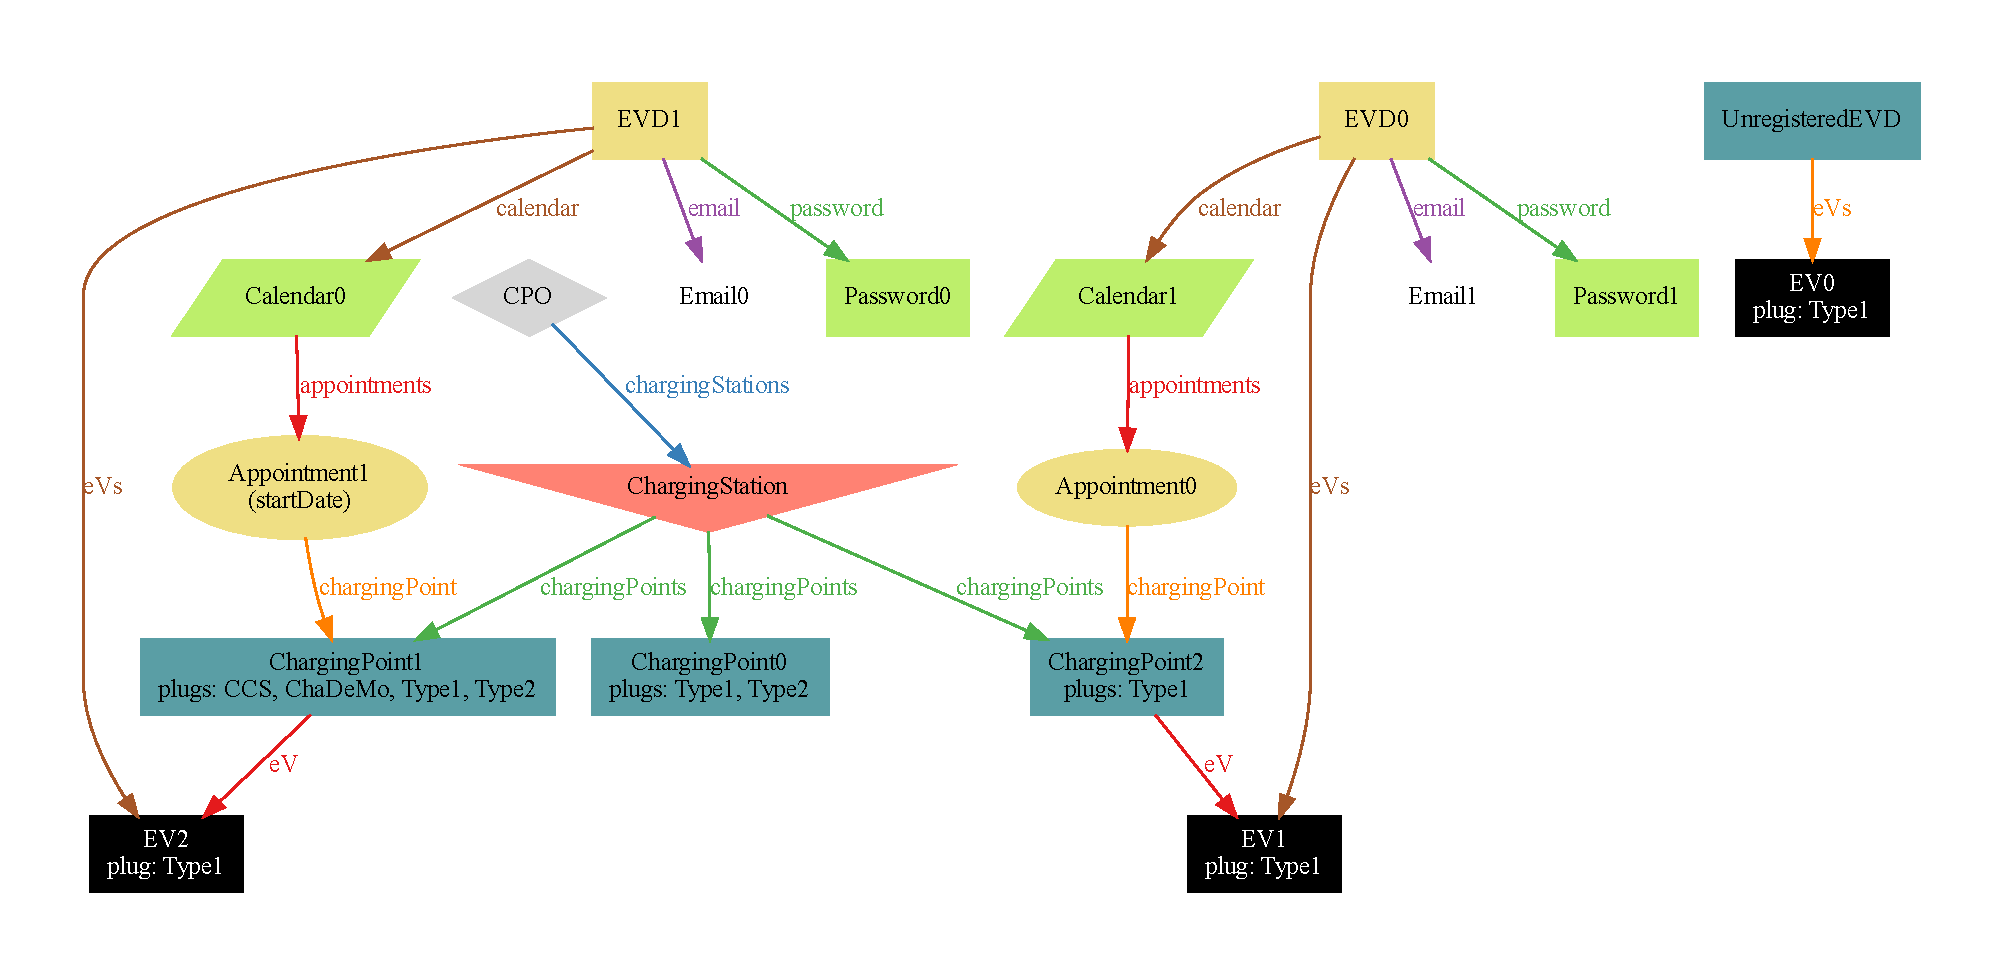
\includegraphics[width=1\linewidth]{graphs/simpleWorld}
			\caption{Simple world Alloy.}
			\label{fig: simple_world_alloy}
		\end{center}
	\end{figure}
\end{sidewaysfigure}

\begin{sidewaysfigure}
	\begin{figure} [H]
		\begin{center}
			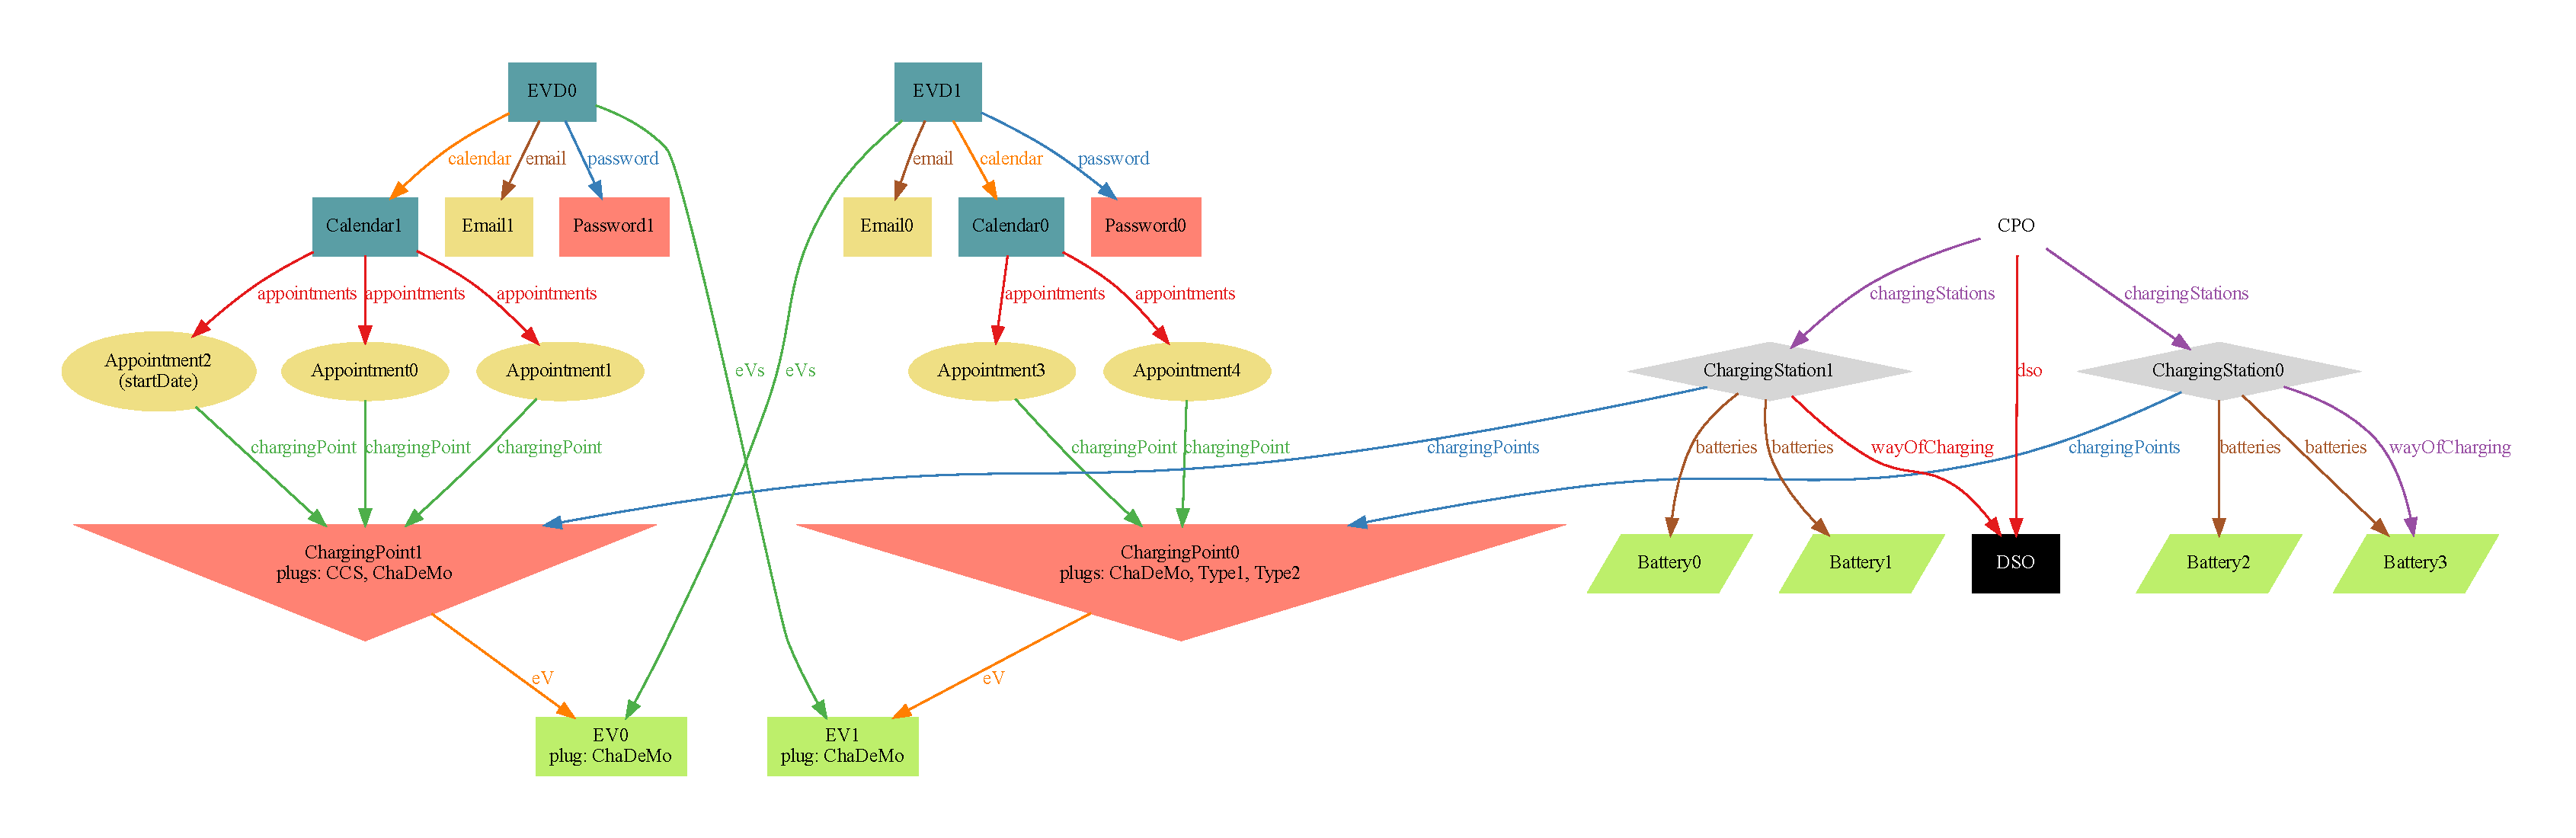
\includegraphics[width=1\linewidth]{graphs/worldWithManyAppointments}
			\caption{More complex world.}
			\label{fig: many_appointments_world_alloy}
		\end{center}
	\end{figure}
\end{sidewaysfigure}



    \chapter{Effort Spent}
    \label{ch:effort_spent}%
    \begin{table}
    \begin{center}
        \caption{Effort spent by each member of the group.}
        \label{tab:effor_spent}
        \begin{tabular}{c|c}
            Member of group & Effort spent \\
            Cela Irfan & \begin{tabular}{c|c}
                             Introduction          & $h$ \\
                             Overall description   & $h$ \\
                             Specific requirements & $h$ \\
                             Formal analysis       & $h$ \\
                             Reasoning             & $h$ \\
            \end{tabular} \\
            Cela Mario & \begin{tabular}{c|c}
                             Introduction          & $h$ \\
                             Overall description   & $h$ \\
                             Specific requirements & $h$ \\
                             Formal analysis       & $h$ \\
                             Reasoning             & $h$ \\
            \end{tabular} \\
            Cogollo Alessandro & \begin{tabular}{c|c}
                                     Introduction          & $h$ \\
                                     Overall description   & $h$ \\
                                     Specific requirements & $h$ \\
                                     Formal analysis       & $h$ \\
                                     Reasoning             & $h$ \\
            \end{tabular} \\
        \end{tabular}
    \end{center}
\end{table}



    \chapter{References}
    \label{ch:references}%
    \section{Paper references}
\label{sec:paper_references}%
\begin{itemize}
    \item \href{https://polimi365-my.sharepoint.com/:b:/g/personal/10685242_polimi_it/EWPABzzjfF9EsgYvSiuvdAIBAz6qnjdfLuPE8kwQSxeyCg?e=6qasKD}{The specification document Assignment RDD AY 2022-2023.pdf}
    \item \href{https://www.platformelectromobility.eu/2022/05/17/ev-charging-how-to-tap-in-the-grid-smartly/}{Platform for Electromobility. EV Charging: How to tap in the grid smartly?}
    \item \href{https://mobilityintegrationsymposium.org/wp-content/uploads/sites/10/2018/11/4A_3_Emob18_024_paper_Filipe_Campos.pdf}{F. Campos, L. Marques, and K. Kotsalos, Electric Vehicle CPMS and Secondary Substation Management. 2nd E-Mobility Power System Integration Symposium,  Stockholm,  Sweden,  15 October 2018. }
    \item \href{https://polimi365-my.sharepoint.com/:b:/g/personal/10685242_polimi_it/EfCXzQWCkK1Lsdtr4suEMp8B7YR3drdGqkArs7hnEx-bqA?e=xy1OTu}{Shu Su, Hui Yan, and Ning Ding. 2018. Machine Learning-Based Charging Network Operation Service Platform Reservation Charging Service System}
    \item \href{https://www.motus-e.org/analisi-di-mercato/settembre-2022-troppa-incertezza-consumatori-preoccupati-non-acquistano/}{September 2022 Market Analysis - MOTUS-E}
\end{itemize}


\section{Used tools}
\label{sec:used_tools}%
\begin{itemize}
    \item \href{https://github.com/}{GitHub} for project versioning
    \item \href{https://staruml.io/}{StarUML} for UML diagrams
    \item \href{https://www.notion.so/}{Notion} for reasoning and notes
    \item \href{https://www.jetbrains.com/idea/}{IntelliJ} as \LaTeX\ editor
    \item \href{https://alloytools.org/}{Alloy} for formal analysis
    \item \href{https://code.visualstudio.com/}{Visual Studio Code} as Alloy editor
\end{itemize}



%-------------------------------------------------------------------------
%	APPENDICES
%-------------------------------------------------------------------------

    \cleardoublepage
    \addtocontents{toc}{\vspace{2em}} % Add a gap in the Contents, for aesthetics
    \appendix


    \chapter{Appendix A}
    \label{ch:appendix_a}%
    If you need to include an appendix to support the research in your thesis, you can place it at the end of the manuscript.
    An appendix contains supplementary material (figures, tables, data, codes, mathematical proofs, surveys, \dots)
    which supplement the main results contained in the previous chapters.


% LIST OF FIGURES
    \listoffigures

% LIST OF TABLES
    \listoftables
    \cleardoublepage
\end{document}
